%!TeX spellcheck=en_US
\documentclass[11pt,
               a4paper,
               bibtotoc,
               idxtotoc,
               headsepline,
               footsepline,
               footexclude,
               BCOR12mm,
               DIV13,
               openany,   % using this removes blank pages around part / chapter starts.
%               oneside    % include this if you have to print only one page per sheet of paper.
               ]
               {scrbook}

%%% SETTINGS

% no word wrapping
%\righthyphenmin=62
%\lefthyphenmin=62
% fewer hyphens
\usepackage{microtype}

% german symbols
\usepackage[utf8]{inputenc}

% strikethrough by \sout
\usepackage[normalem]{ulem}

% insert graphics
\usepackage{graphicx}
% more flexible figures e.g. graphics with captions beside them
\usepackage{floatrow}
% more flexible captions.
% Use \captionsetup{options} to configure,
% use it in an environment for local setup
\usepackage{caption}
% subfigures (see template):
\usepackage{subcaption}

% more control of enumerations and itemizations
\usepackage{enumitem}
% less space between items
\setlist[itemize]{itemsep=0cm}
\setlist[enumerate]{itemsep=0cm}
% more customizeable tables (e.g. multiple lines per cell)
\usepackage{tabularx}
% fix for vertical centering
\usepackage{ragged2e}
\renewcommand\tabularxcolumn[1]{>{\Centering}m{#1}}
% column types with multiple lines and formatting
\usepackage{array}
\newcolumntype{C}{>{\centering\arraybackslash}X}
\newcolumntype{R}{>{\raggedleft\arraybackslash}X}
\newcolumntype{L}{>{\raggedright\arraybackslash}X}
% merge multiple rows \multirow{2}{*}{bla} & \\ &
\usepackage{multirow}
% activate for tables with page breaking
%\usepackage{ltablex}
% fix for table movement and itemizations
%\keepXColumns

% fix for dynamics spaces after custom commands
\usepackage{xspace}

% tabbing: use with \tab
\usepackage{tabto}
\TabPositions{4cm}

%% fancy math
% propper matrices, underbrace text
%\usepackage{amsmath}
\usepackage{mathtools}
% special symbols e.g. squares
\usepackage{amssymb}

%% plotting
\usepackage{pgfplots}
\usepgfplotslibrary{fillbetween}

%%Settings for code
% code placement right there
\usepackage{float}
% code coloring
\usepackage{xcolor}
% code listing
\usepackage{listings}

% flexible multi column style
\usepackage{multicol}

% graphs
\usepackage{tikz}
\usetikzlibrary{shapes.geometric, arrows}
% define some elements
\tikzstyle{startstop} = [rectangle, rounded corners, minimum width=3cm, minimum height=1cm,text centered, draw=black, fill=blue!30]
\tikzstyle{arrow} = [thick,->,>=stealth]

% Some code highlighting styles you can use with lstlistings
% C++ code style similar to default eclipse
\lstdefinestyle{eclipse-cpp} {
    captionpos=b,
    language=C++,
    otherkeywords={final},
    basicstyle=\footnotesize,
    numbers=left,
    numberstyle=\small,
    showstringspaces=false,
    tabsize=2,
    frame=single,
    breaklines=true,
    keywordstyle=\bfseries\color[RGB]{127,0,85},
    identifierstyle=\color[RGB]{0,0,192},
    stringstyle=\color[RGB]{42,0,255},
    commentstyle=\color[RGB]{63,127,95},
}

% If no highlighting is intended
\lstdefinestyle{plain}{
}

% fancy algorithms (see template)
\usepackage[ruled, vlined, linesnumbered]{algorithm2e}
\DontPrintSemicolon
\SetKw{KwBy}{by}
\SetKw{KwAnd}{and}

% clickable links and clickable table of content <3
% Options: links with linebreaks
\PassOptionsToPackage{hyphens}{url}\usepackage[bookmarks=false]{hyperref}
\hypersetup{
    colorlinks,
    citecolor=black,
    filecolor=black,
    linkcolor=black,
    urlcolor=black
}
% Alterations to labels used by \autoref{}: Capitalize everyything
\def\chapterautorefname{Chapter}
\def\sectionautorefname{Section}
\def\subsectionautorefname{Subsection}
\def\algorithmautorefname{Algorithm}
\def\subfigureautorefname{Figure}
% for fully custon stuff use:
% \hyperref[custom:foo]{Custom~\ref*{custom:foo}}


\usepackage{lipsum} % for filling pages with stuff

% -------------------------------------------------------------------------------
% --------------------------------- Thesis Info ---------------------------------
% -------------------------------------------------------------------------------

% set title, authors and stuff for the cover
% docytype needs xspace because it is used within text.
\def\doctype{Bachelor's Thesis\xspace}
%\def\doctype{Master's Thesis\xspace}
%\def\doctype{Guided Research\xspace}
%\def\doctype{Interdisciplinary Project\xspace}
\def\studyProgram{Informatics}
\def\title{Implementing and benchmarking Discrete Element Method simulator using AutoPas}
% don't try translate every technical term if it would sound off
\def\titleGer{Implementierung und Benchmarking von Discrete Element Method Simulator unter Anwendung von AutoPas}
\def\author{Joon Kim}
% Prof
\def\supervisor{Univ.-Prof. Dr. Hans-Joachim Bungartz}
% PhD Candidate
\def\advisor{Manish Kumar Mishra, M.Sc.}
\def\date{Date of Submission}

\begin{document}
\frontmatter
% -------------------------------------------------------------------------------
% ---------------------------------- COVERPAGE ----------------------------------
% -------------------------------------------------------------------------------

% correct BCOR - undo at the end !!!
\def\bcorcor{0.15cm}
\addtolength{\hoffset}{\bcorcor}
\thispagestyle{empty}
\vspace{4cm}
\begin{center}
    
\includegraphics[width=4cm]{templateStuff/tumlogo.pdf}\\[5mm]
    \huge SCHOOL OF COMPUTATION, INFORMATION AND TECHNOLOGY\\[5mm]
    \large DER TECHNISCHEN UNIVERSITÄT MÜNCHEN\\[24mm]

    {\Large \doctype in \studyProgram}\\[20mm]
    {\huge\bf \title\par}
    \vspace{15mm}
    {\LARGE  \author}
\end{center}

\cleardoubleemptypage

% -------------------------------------------------------------------------------
% ---------------------------------- TITLEPAGE ----------------------------------
% -------------------------------------------------------------------------------

\def\bcorcor{0.15cm}
\addtolength{\hoffset}{\bcorcor}
\thispagestyle{empty}
\vspace{10mm}
\begin{center}
    
\includegraphics[width=4cm]{templateStuff/tumlogo.pdf}\\[5mm]
	\huge SCHOOL OF COMPUTATION, INFORMATION AND TECHNOLOGY\\[5mm]
	\large DER TECHNISCHEN UNIVERSITÄT MÜNCHEN\\[24mm]
	{\Large \doctype in \studyProgram}\\[20mm]
	{\LARGE\bf \title}\\[10mm]
	{\LARGE\bf \titleGer}\\[10mm]
	\begin{tabular}{ll}
		\Large Author:      	& \Large \author \\[2mm]
		\Large Supervisor:  	& \Large \supervisor\\[2mm]
		\Large Advisor:			& \Large \advisor\\[2mm]
		\Large Date:       		& \Large \date
	\end{tabular}
\end{center}

% undo BCOR correction
\addtolength{\hoffset}{\bcorcor}
\newpage

% -------------------------------------------------------------------------------
% ---------------------------------- DISCLAIMER ---------------------------------
% -------------------------------------------------------------------------------

\cleardoubleemptypage

\thispagestyle{empty}
\vspace*{0.7\textheight}
\noindent
I confirm that this \MakeLowercase{\doctype} is my own work and I have documented all sources and material used.\\

\vspace{15mm}
\noindent
Munich, \date \hspace{5cm} \author
\cleardoubleemptypage

% -------------------------------------------------------------------------------
% ------------------------------- ACKNOWLEDGEMENTS ------------------------------
% -------------------------------------------------------------------------------

\phantomsection
\addcontentsline{toc}{chapter}{Acknowledgements}
\vspace*{2cm}
\begin{center}
    {\Large \bf Acknowledgements}
\end{center}
\vspace{1cm}

\lipsum[1]

\cleardoublepage

% -------------------------------------------------------------------------------
% ---------------------------------- ABSTRACT -----------------------------------
% -------------------------------------------------------------------------------

\phantomsection
\addcontentsline{toc}{chapter}{Abstract}
\vspace*{2cm}
\begin{center}
    {\Large \bf Abstract}
\end{center}
\vspace{1cm}

\lipsum[2]

\cleardoublepage

\phantomsection
\addcontentsline{toc}{chapter}{Zusammenfassung}
\vspace*{2cm}
\begin{center}
    {\Large \bf Zusammenfassung}
\end{center}
\vspace{1cm}

\lipsum[2]

\cleardoublepage

% -------------------------------------------------------------------------------
% ------------------------------ TABLE OF CONTENTS ------------------------------
% -------------------------------------------------------------------------------

\tableofcontents
\thispagestyle{empty}
\cleardoubleemptypage

% -------------------------------------------------------------------------------
% --------------------------------- MAIN MATTER ---------------------------------
% -------------------------------------------------------------------------------

\mainmatter
\part{Introduction}
\label{sec:introduction}
The Discrete Element Method (DEM) usually attempts to gain microscopic understanding by modeling macroscopic specific behaviors. By assuming contact laws from physics and the rigidity of granular bodies, it simulates the interactions of samples. 

DEM has been widely used in the field of granular science due to its many advantages  when compared to a continuous modeling of granular materials: It is simple physics and provides insights into local quantities of individual granular bodies that could be out of reach in case of continuous modeling.

This thesis focuses on the application of AutoPas, a high-performance, auto-tuned particle simulation library for N-body systems, building a DEM simulator and benchmarking different experimental results.

\part{Theory}
\chapter{Discrete spherical particle model}
\label{sec:discrete_spherical_particle_model}

The body shape of granular materials that are subjects of DEM simulations could be various. For example, sand has its specific cristal shape, which might differ from other grains such as corn or salt. 
To simplify the modeling and implementation, we assume the spherical shape of the granular units, in which the mass is uniformly distributed over its volumne.
Moreover, soft and elastic unit can undergo deformations under stress. Again, for simplicity reasons, we ignore such elastic/plastic deformations and assume an unchangable spherical shape of particles.

Ignoring the complicated stress distribution, the interaction forces in DEM only rely on the overlap between colliding two particles. As a consequence, the produced results below are of the same quality as the simplified modeling decision made here. 

 \begin{figure}[H] % [H] for HERE
	\centering
	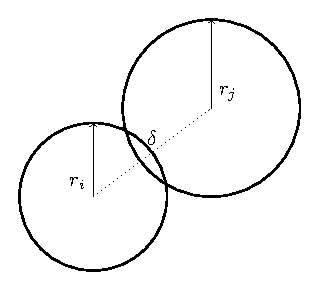
\includegraphics[width=.3\columnwidth]{figures/discrete_spherical_particle_model.pdf}
	\caption[Example Figure]{Two spherical particles in contact with overlap $\delta$ \\
		\tiny{Source: \cite{Luding2008}}}
	\label{fig:discrete_spherical_particle_model} % labels always have to be placed after the caption
\end{figure}

\chapter{Equations of Motion}
The dynamics of granular particles can be expressed with Newton's equations, which can be reduced to a system of ordinary differential equations of translational and rotational  motion:
\begin{equation}
	m_i \frac{\mathrm{d}^2}{\mathrm{d}t^2} x_i = f_{contact} + f_{global}, \quad \text{and} \quad
	I_i \frac{\mathrm{d}^2}{\mathrm{d}t^2} \varphi_i = q_{contact} + q_{global}
	\label{equations_of_motion}
\end{equation}
with the mass $m_i$  of particle $i$ and its position $x_i$. The $f_{contact}$ can be obtained by the sum of all contact forces directed to particle $i$ as we assume existing interaction force when contact between two particles is present:
\begin{equation}
f_{contact} = \sum_{j \in C_{i}, i \neq j}^{} f_{ij},
\end{equation}
with $C_i$ being the set of all particles in contact with $i$. In case of present walls or reflective boundary conditions (BC), the forces ensuring such BC should be added into $f_{contact}$.
The global force $f_{global}$ expresses a force that applies to all particles in a system e.g. gravity or background friction.

Similar applies to the equations for rotational motion: the moment of inertia $I_i$ of particle $i$, which can be reduced to the closed form solution $I_i = \frac{2}{5} m_i  r_i^2$ due to the aforementioned spherical body assumption, and its angular position $\varphi_i$. The $q_{contact}$ expresses the sum of all torques rising from its contacts with other particles:
\begin{equation}
	q_{contact} = \sum_{j \in C_{i}, i \neq j}^{} q_{ij},
\end{equation}
Such torques  can rise from a tangential force, rolling and torsion as will be discussed later.
Similar to $f_{global}$, the global torque $q_{global}$, e.g. background friction, is subjected to all particles in the system.

For a $D$-dimensional simulation, each particle has $D$ translational degrees of freedom (DF), due to the $D$-dimensional coordinate axes, and $\frac{D(D-1)}{2}$ rotational DF, due to the number of possible rotational planes e.g. $xy$, $yz$, and $xz$ planes. This results in  $D + D(D-1)/2$ ODEs for each particle, that are coupled due to the tangential force, which also affects the tangential torque.

For approximating the solutions of these ODEs, numerical integrators can be applied, which will be presented next.


\chapter{Time Discretization}
Due to practical reasons, the aforementioned problem that is posed on a continuous time interval has to be transformed to a problem that is posed on discrete time steps. This brings the necessity of a numeric integrator that is applied to compute the new quantities for translational and rotational motion.

\section{The Integration Method of Störmer-Verlet}
In the context of translational motion, the task is to compute the new positions and velocities of the particles from the old positions, old velocities, and the relevant forces. From a variety of differently accurate and complex numerical integrators, the focus of our simulation lies on observing developments of macroscopic quantities e.g. Energy, Distribution of Particles and Pressure. This application makes high-order integrators such as Runge-Kutta rather unsuitable due to its bad scalability in time and memory. Instead, a second order symplectic integrator such as Velocity-Störmer-Verlet seems more promising due to its capability to capture long-time patterns well. The formulas for Störmer-Verlet is presented in the following.

\begin{equation}
	x_i(t_{n+1}) = x_i(t_n) + \Delta t \cdot v_i(t_n) + \frac{(\Delta t)^2 F_i(t_n)}{2m_i}, 
\end{equation}
\begin{equation}
	v_i(t_{n+1}) = v_i(t_n) + \Delta t \cdot \frac{F_i(t_n) + F_i(t_{n+1})}{2m_i},
\end{equation}
with the position $x_i$, the velocity $v_i$, the mass $m_i$, and the force $F_i$ of particle $i$ and the old time step $t_n$ and the new time step $t_{n+1}$ with $\Delta t = t_{n+1} - t_n$.

\section{The Integration Method of Explicit Euler}
In the context of rotational motion, we can simplify the integration due to following reasons. Because of the assumption of the spherical particle model, the relevance of orientation, which corresponds to the position in the translational motion, disappears. Moreover, our main interest lies on observing the development of rotational motion rather than calculating accurate macroscopic quantities such as the rotational energy. This requirement allows us to use a simple first-order integrator of Explicit Euler with its computational and spacial advantages:

\begin{equation}
	w_i(t_{n+1}) = w_i(t_n) + \Delta t \cdot \frac{q_i(t_n)}{I_i},
\end{equation}

with the angular velocity $w_i$, the torque $q_i$, and the moment of Inertia $I_i$ of particle $i$.

\chapter{Contact Force Laws}

The interaction force models can be divided into two main classes: normal and tangential forces. Here, we introduce the force models presented by \cite{Luding2008} that show great similarities to classical mechanics from physics.

\section{Normal Contact Force Laws}
\subsection{Linear Normal Contact Model}
The model used for expressing the normal force between particles is the maxwell linear spring dashpot model, which consists of a spring generating a linear repulsive force and a damper realizing a dissipative viscosity.

 \begin{figure}[H] % [H] for HERE
	\centering
	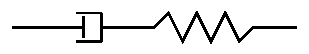
\includegraphics[width=.5\columnwidth]{figures/maxwell_spring_dashpot.pdf}
	\caption[Example Figure]{Maxwell spring dashpot model with a dashpot and a spring placed in series}
	\label{fig:maxwell_spring_dashpot} % labels always have to be placed after the caption
\end{figure}

This model becomes active only if and only if the overlap $\delta$ between two particles is positive, which can be computed as the sum of the radii of the particles subtracted by their distance:

\begin{equation}
	\delta_{ij} = (r_i + r_j) - \lVert \mathbf{x_i} -\mathbf{ x_j} \rVert_2 = \delta_{ji} 
	\label{overlap_equation}
\end{equation}

with $r$ being the radius of the corresponding particle.
As this model expresses force in the normal direction, which is parallel to the branch vector $\mathbf{l_{ji}}$ pointing from center position of particle $j$ to $i$, the unit vector $\mathbf{n_{ji}}$ in the normal direction should additionally be computed:

\begin{equation}
	\mathbf{l_{ji}} =  \mathbf{x_i} - \mathbf{x_j}, \quad \mathbf{n_{ji}} =\frac{\mathbf{l_{ij}}}{\lVert \mathbf{l_{ij}} \rVert_2}
\end{equation}

For every contact with positive overlap $\delta$, the rising normal force $f_{ji}^n$ on particle $i$ from particle $j$ can be computed by taking into account the repulsion of the spring and the dissipation of the damper (see Figure~\ref{fig:maxwell_spring_dashpot}):

\begin{align}
	f_{ji}^n &= f^n_{elastic} + f^n_{dissipative}, \label{linear_normal_contact_model_equation1} \\
	f^n_{elastic} &= k^n\delta, \quad f^n_{dissipative} = - \gamma_n v_{ji}^n, \label{linear_normal_contact_model_equation2} \\
	v_{ji}^n &= \mathbf{v_{ji}} \cdot \mathbf{n_{ji}} = (\mathbf{v_i} - \mathbf{v_j}) \cdot \mathbf{n_{ji}}. \label{linear_normal_contact_model_equation3}
\end{align}



with the spring stiffness $k^n$, the viscous damping coefficient $\gamma_n$, and the relative velocity in normal direction $v_{ji}^n$. The negative sign of the term $-\gamma_n v_{ji}^n$ explains the damping effect, reducing the amount of force according to the damping coefficient $\gamma_n$.

\begin{figure}[H]
	\centering
	% First figure
	\begin{center}
		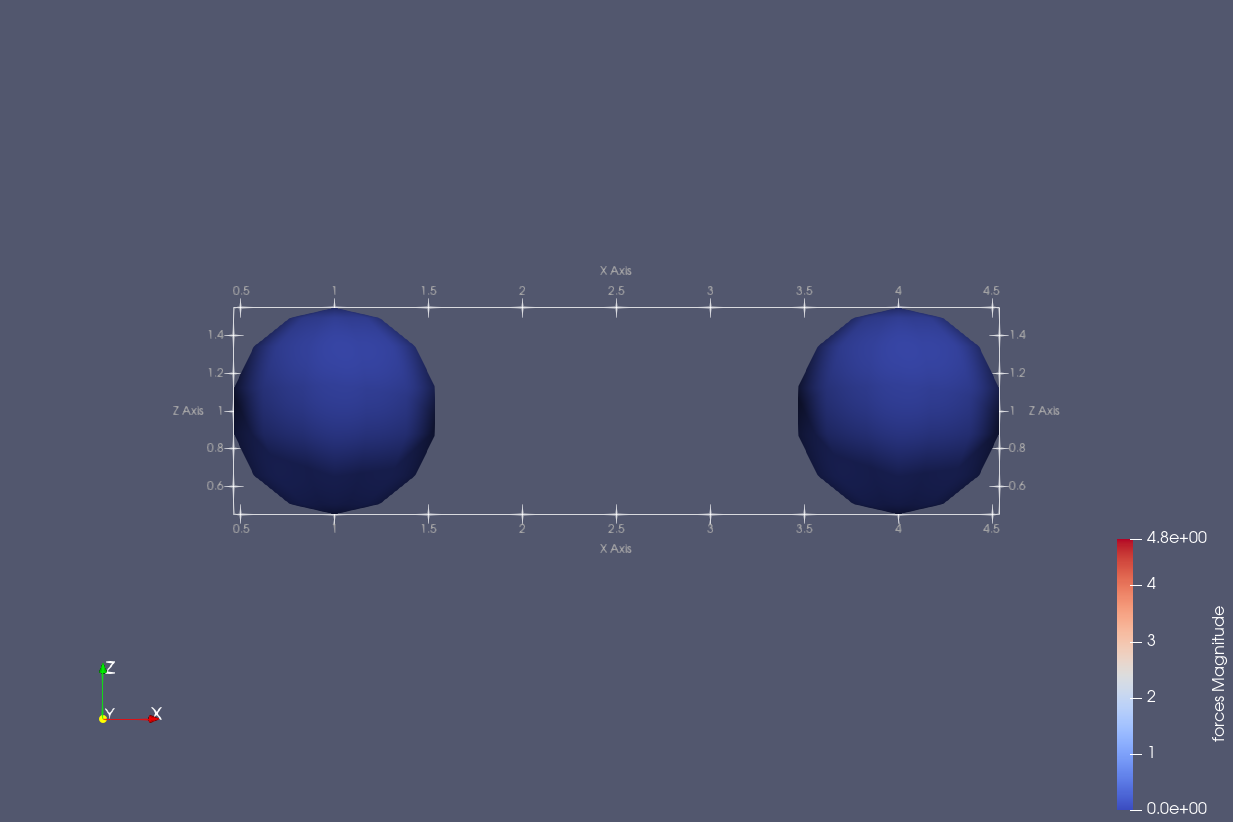
\includegraphics[width=0.6\textwidth]{figures/contactForceLaws/linearNormalContactModel/simple_collision_two_particles_centered.0000.png}
		\\ (a) Initial State % Subcaption directly
	\end{center}
	
	% Second figure
	\begin{center}
		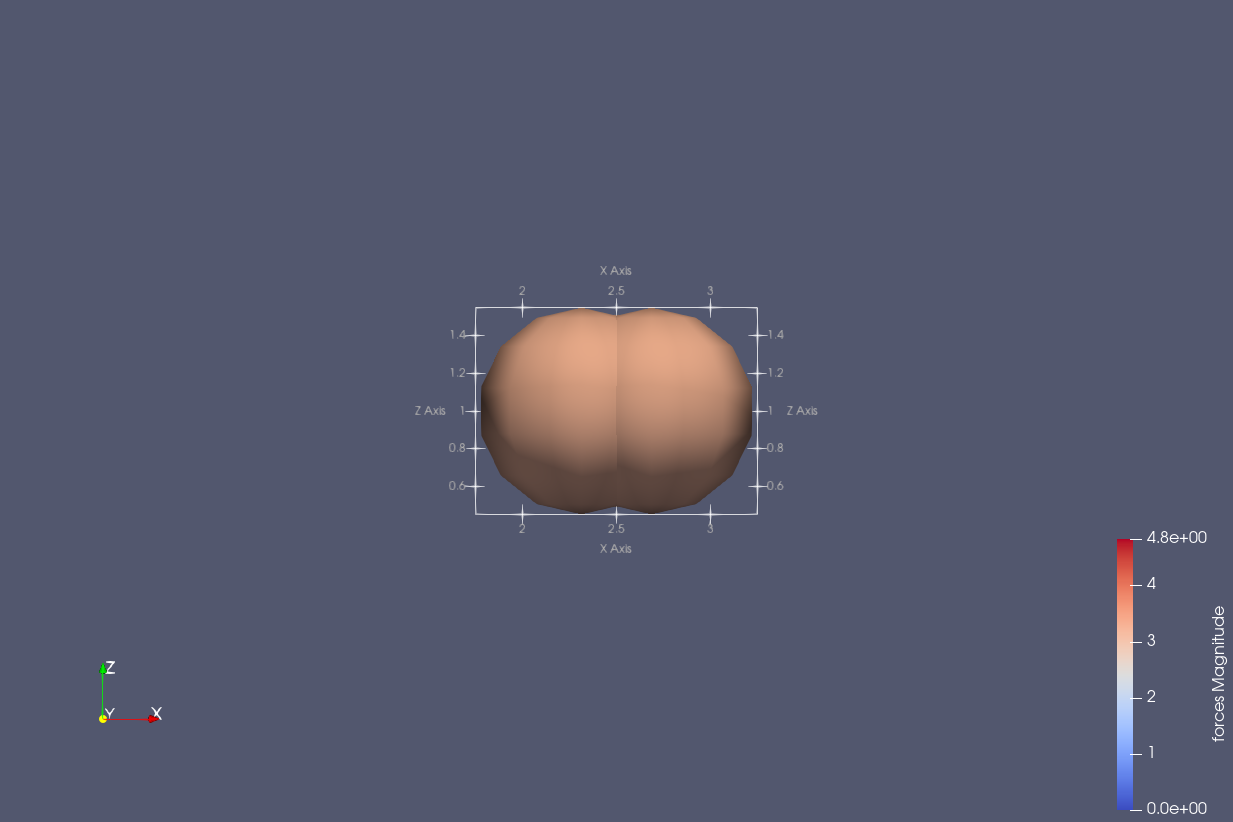
\includegraphics[width=0.6\textwidth]{figures/contactForceLaws/linearNormalContactModel/simple_collision_two_particles_centered.0044.png}
		\\ (b) In Contact % Subcaption directly
	\end{center}
	
	% Shared caption
	\caption[Combined Caption]{Simple simulation of linear normal contact force with a collision of two particles $i$ (right), $j$ (left), color scaled by $\lVert f^n_{ji} \rVert$. Simulation parameters of the initial state: $r_i = r_j = 0.5$, $v^n_{ji} = 6$. (a) Initial state of the particles. (b) State of the particles in contact.}
	\label{fig:combined_linear_normal_contact_model}
\end{figure}

\begin{figure}[H]
	\centering
	\begin{minipage}[t]{0.65\textwidth}
		\centering
		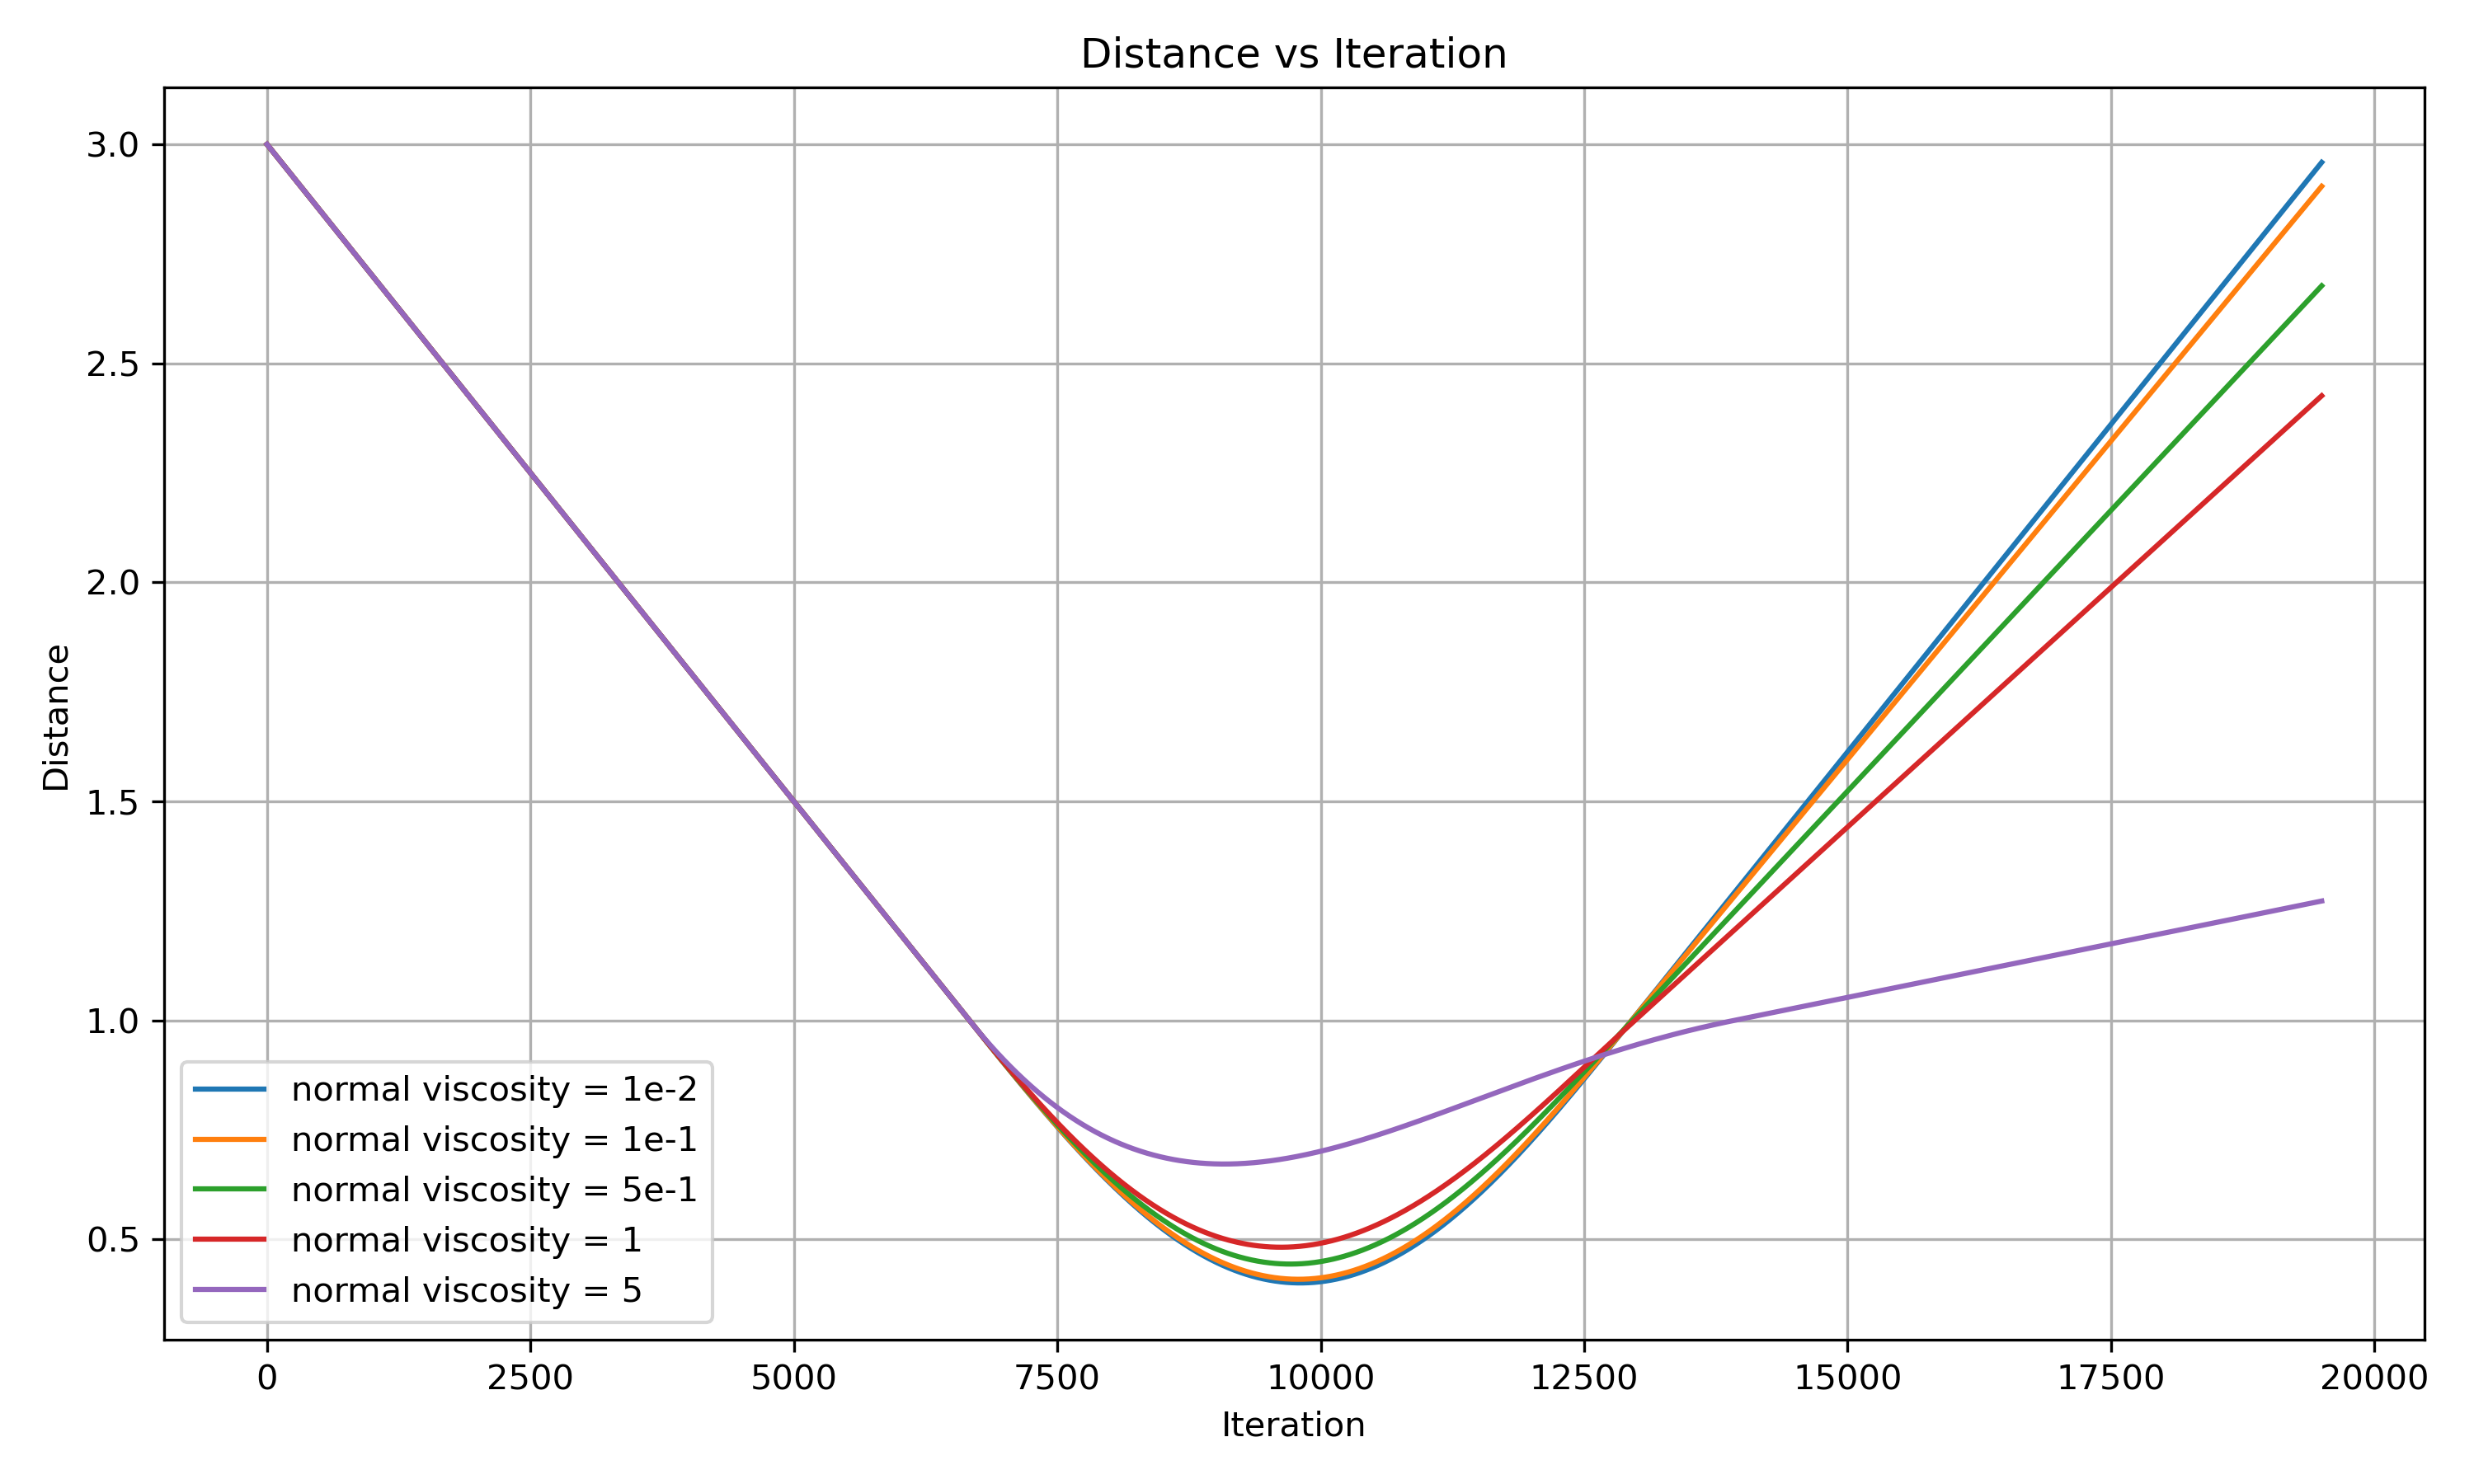
\includegraphics[width=\textwidth]{figures/contactForceLaws/linearNormalContactModel/Distance vs Iterationsimple_collision_two_particles_statistics_stiffness_50_viscosity_1e-2.png}
	\end{minipage}
	
		\vspace{0.5cm} % Add vertical spacing between rows
		
	\begin{minipage}[t]{0.65\textwidth}
		\centering
		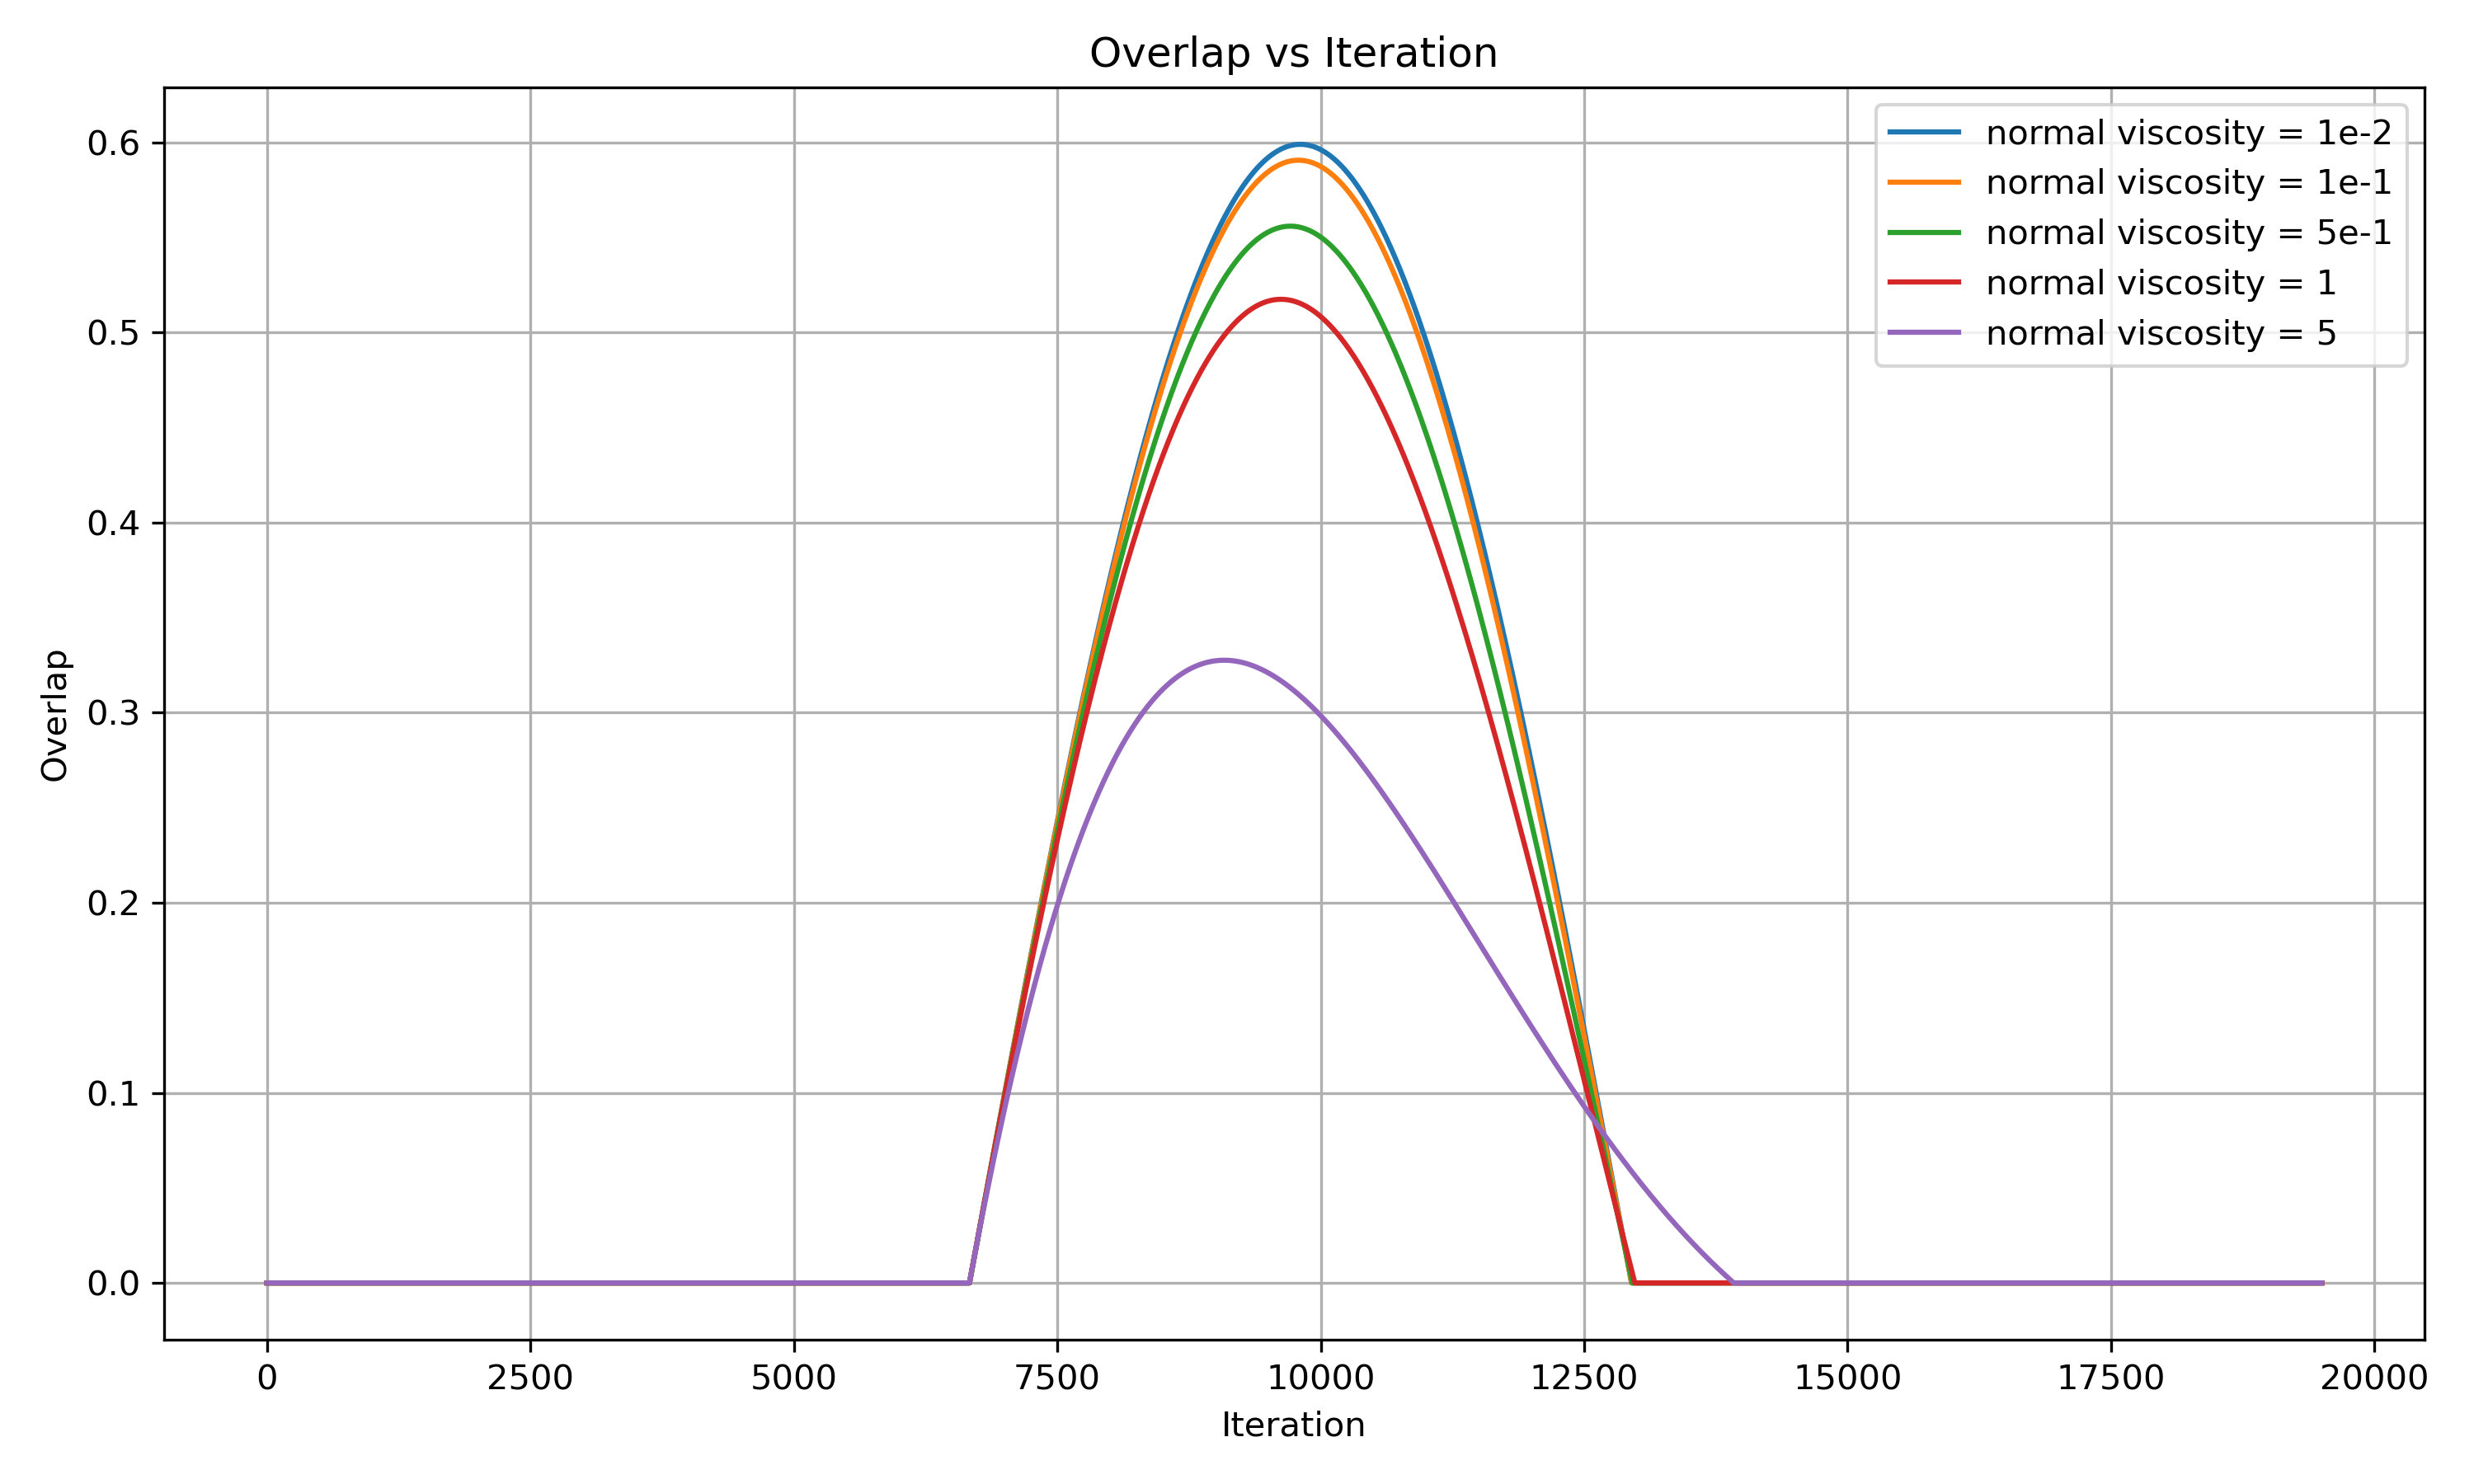
\includegraphics[width=\textwidth]{figures/contactForceLaws/linearNormalContactModel/Overlap vs Iterationsimple_collision_two_particles_statistics_stiffness_50_viscosity_1e-2.png}
	\end{minipage}
	
	\vspace{0.5cm} % Add vertical spacing between rows
	
	% Lower center figure
	\begin{minipage}[t]{0.65\textwidth}
		\centering
		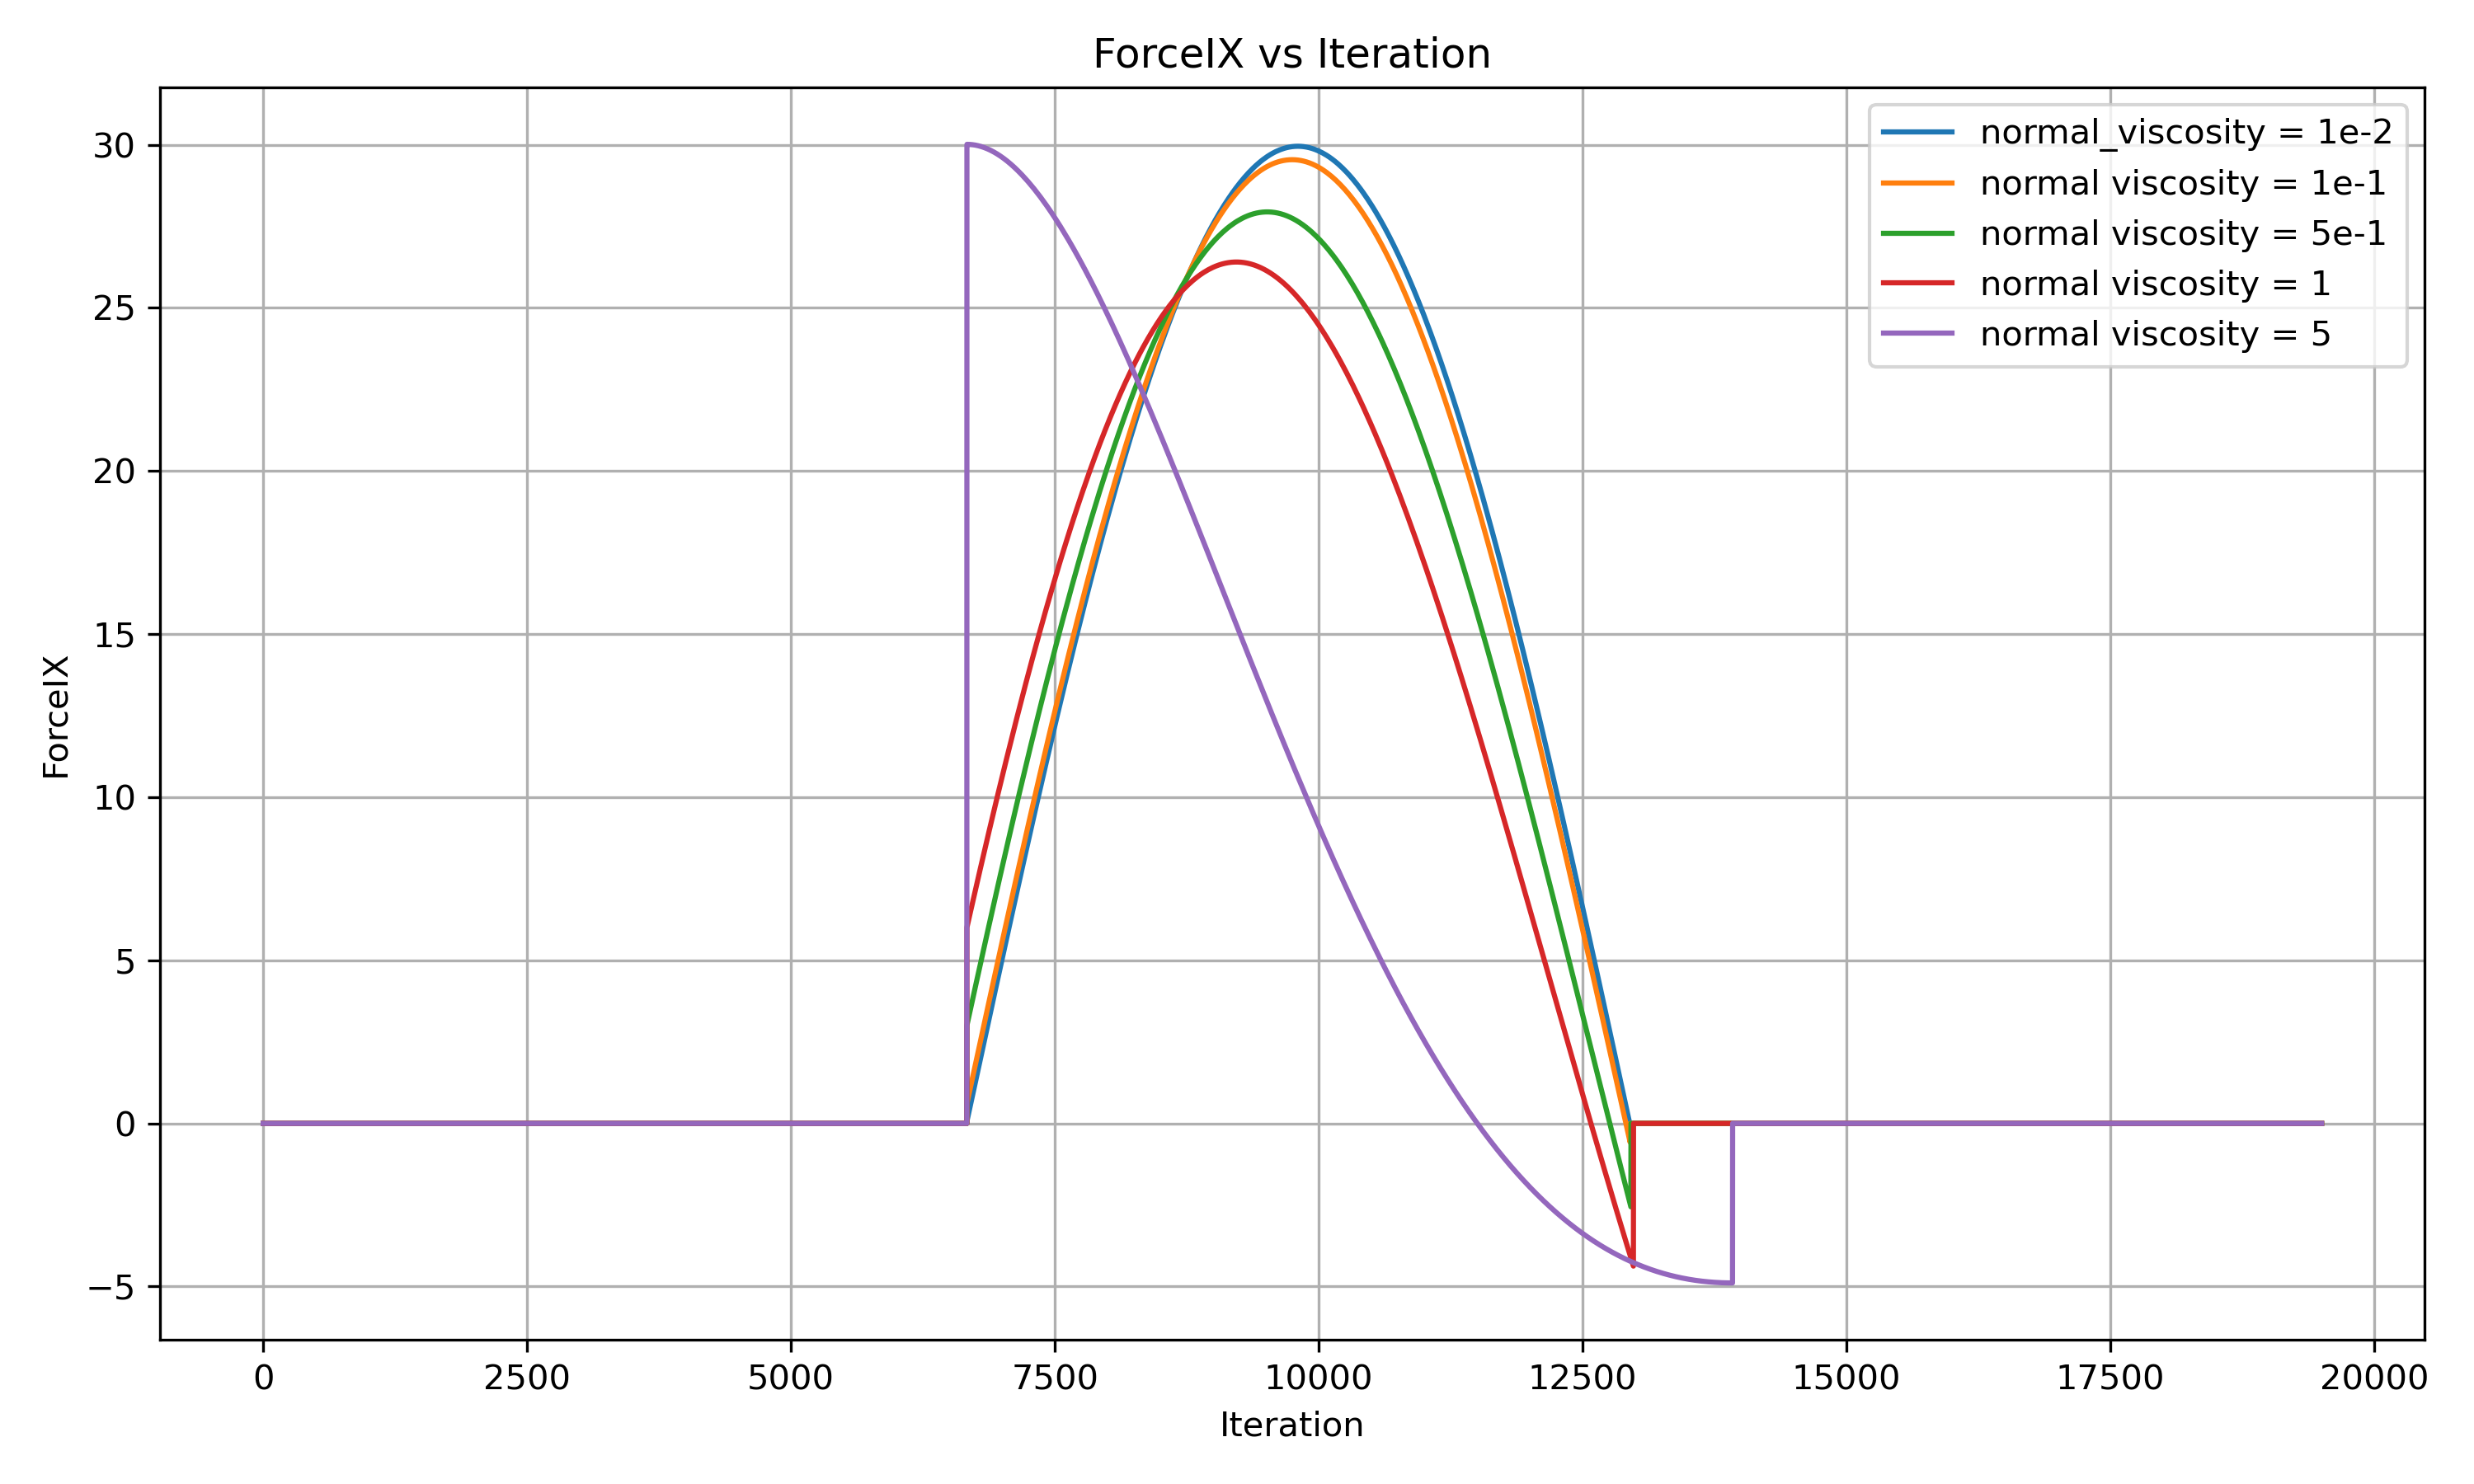
\includegraphics[width=\textwidth]{figures/contactForceLaws/linearNormalContactModel/ForceIX vs Iterationsimple_collision_two_particles_statistics_stiffness_50_viscosity_1e-2.png}
	\end{minipage}
	
	% Shared caption
	\caption[Combined Caption]{Development of distance ($\lVert x_i - x_j \rVert_2$ ), overlap ($\delta$), and force ($f^n_{ji}$ over time in scenario described in Figure~\ref{fig:combined_linear_normal_contact_model}. Simulation parameters: $k^n$ = 50, $\gamma_n \in $ \{0.01, 0.1, 0.5, 1, 5\}, $\Delta t = 5 \cdot 10^{-5}$, number of total iterations = 20000 (a) Distance between particles $i$ and $j$ vs Iteration. (b) Overlap $\delta$ vs Iteration. (c) Linear normal force $f^n_{ji}$ vs Iteration .}
	\label{fig:Distance_Overlap_Force_plots}
\end{figure}

\begin{figure}[H]
	\centering
	% First figure
	\begin{center}
		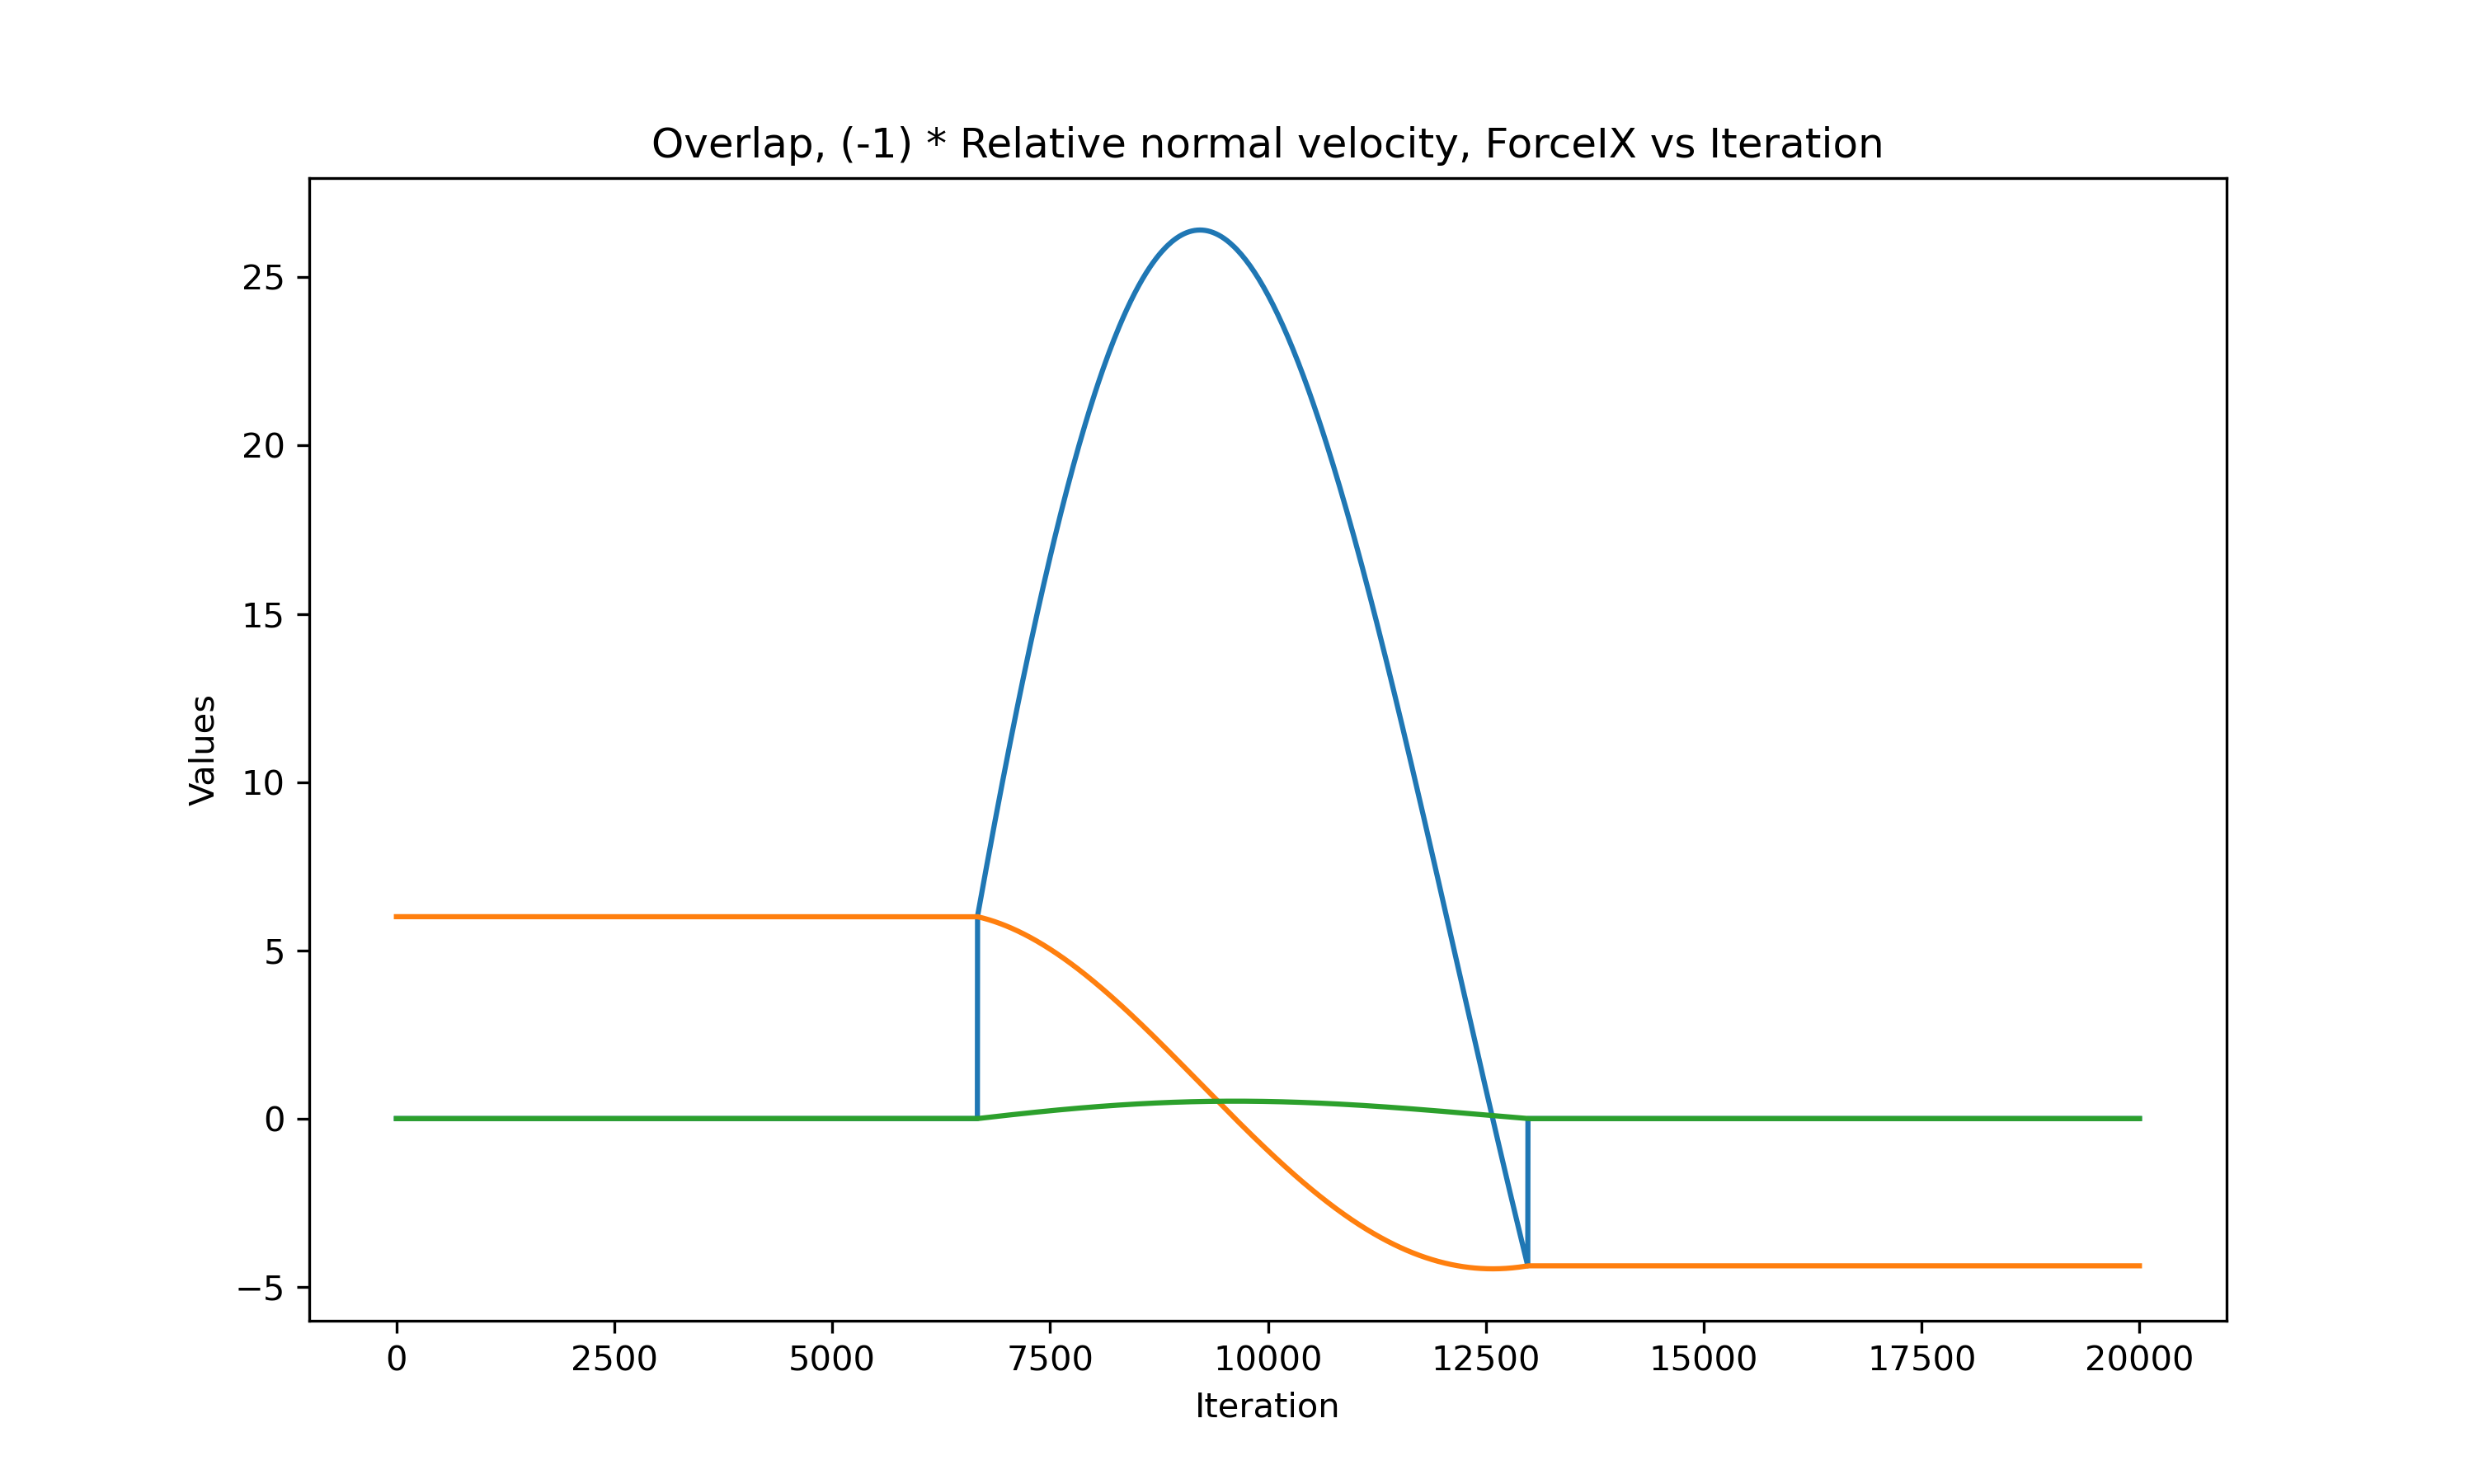
\includegraphics[width=0.65\textwidth]{figures/contactForceLaws/linearNormalContactModel/Overlap, Relative normal velocity vs Iteration simple_collision_two_particles_statistics_stiffness_50_viscosity_1e-2viscosity_1.png}
		\\ (a) $\gamma_n = 1$ % Subcaption directly
	\end{center}
	
	% Second figure
	\begin{center}
		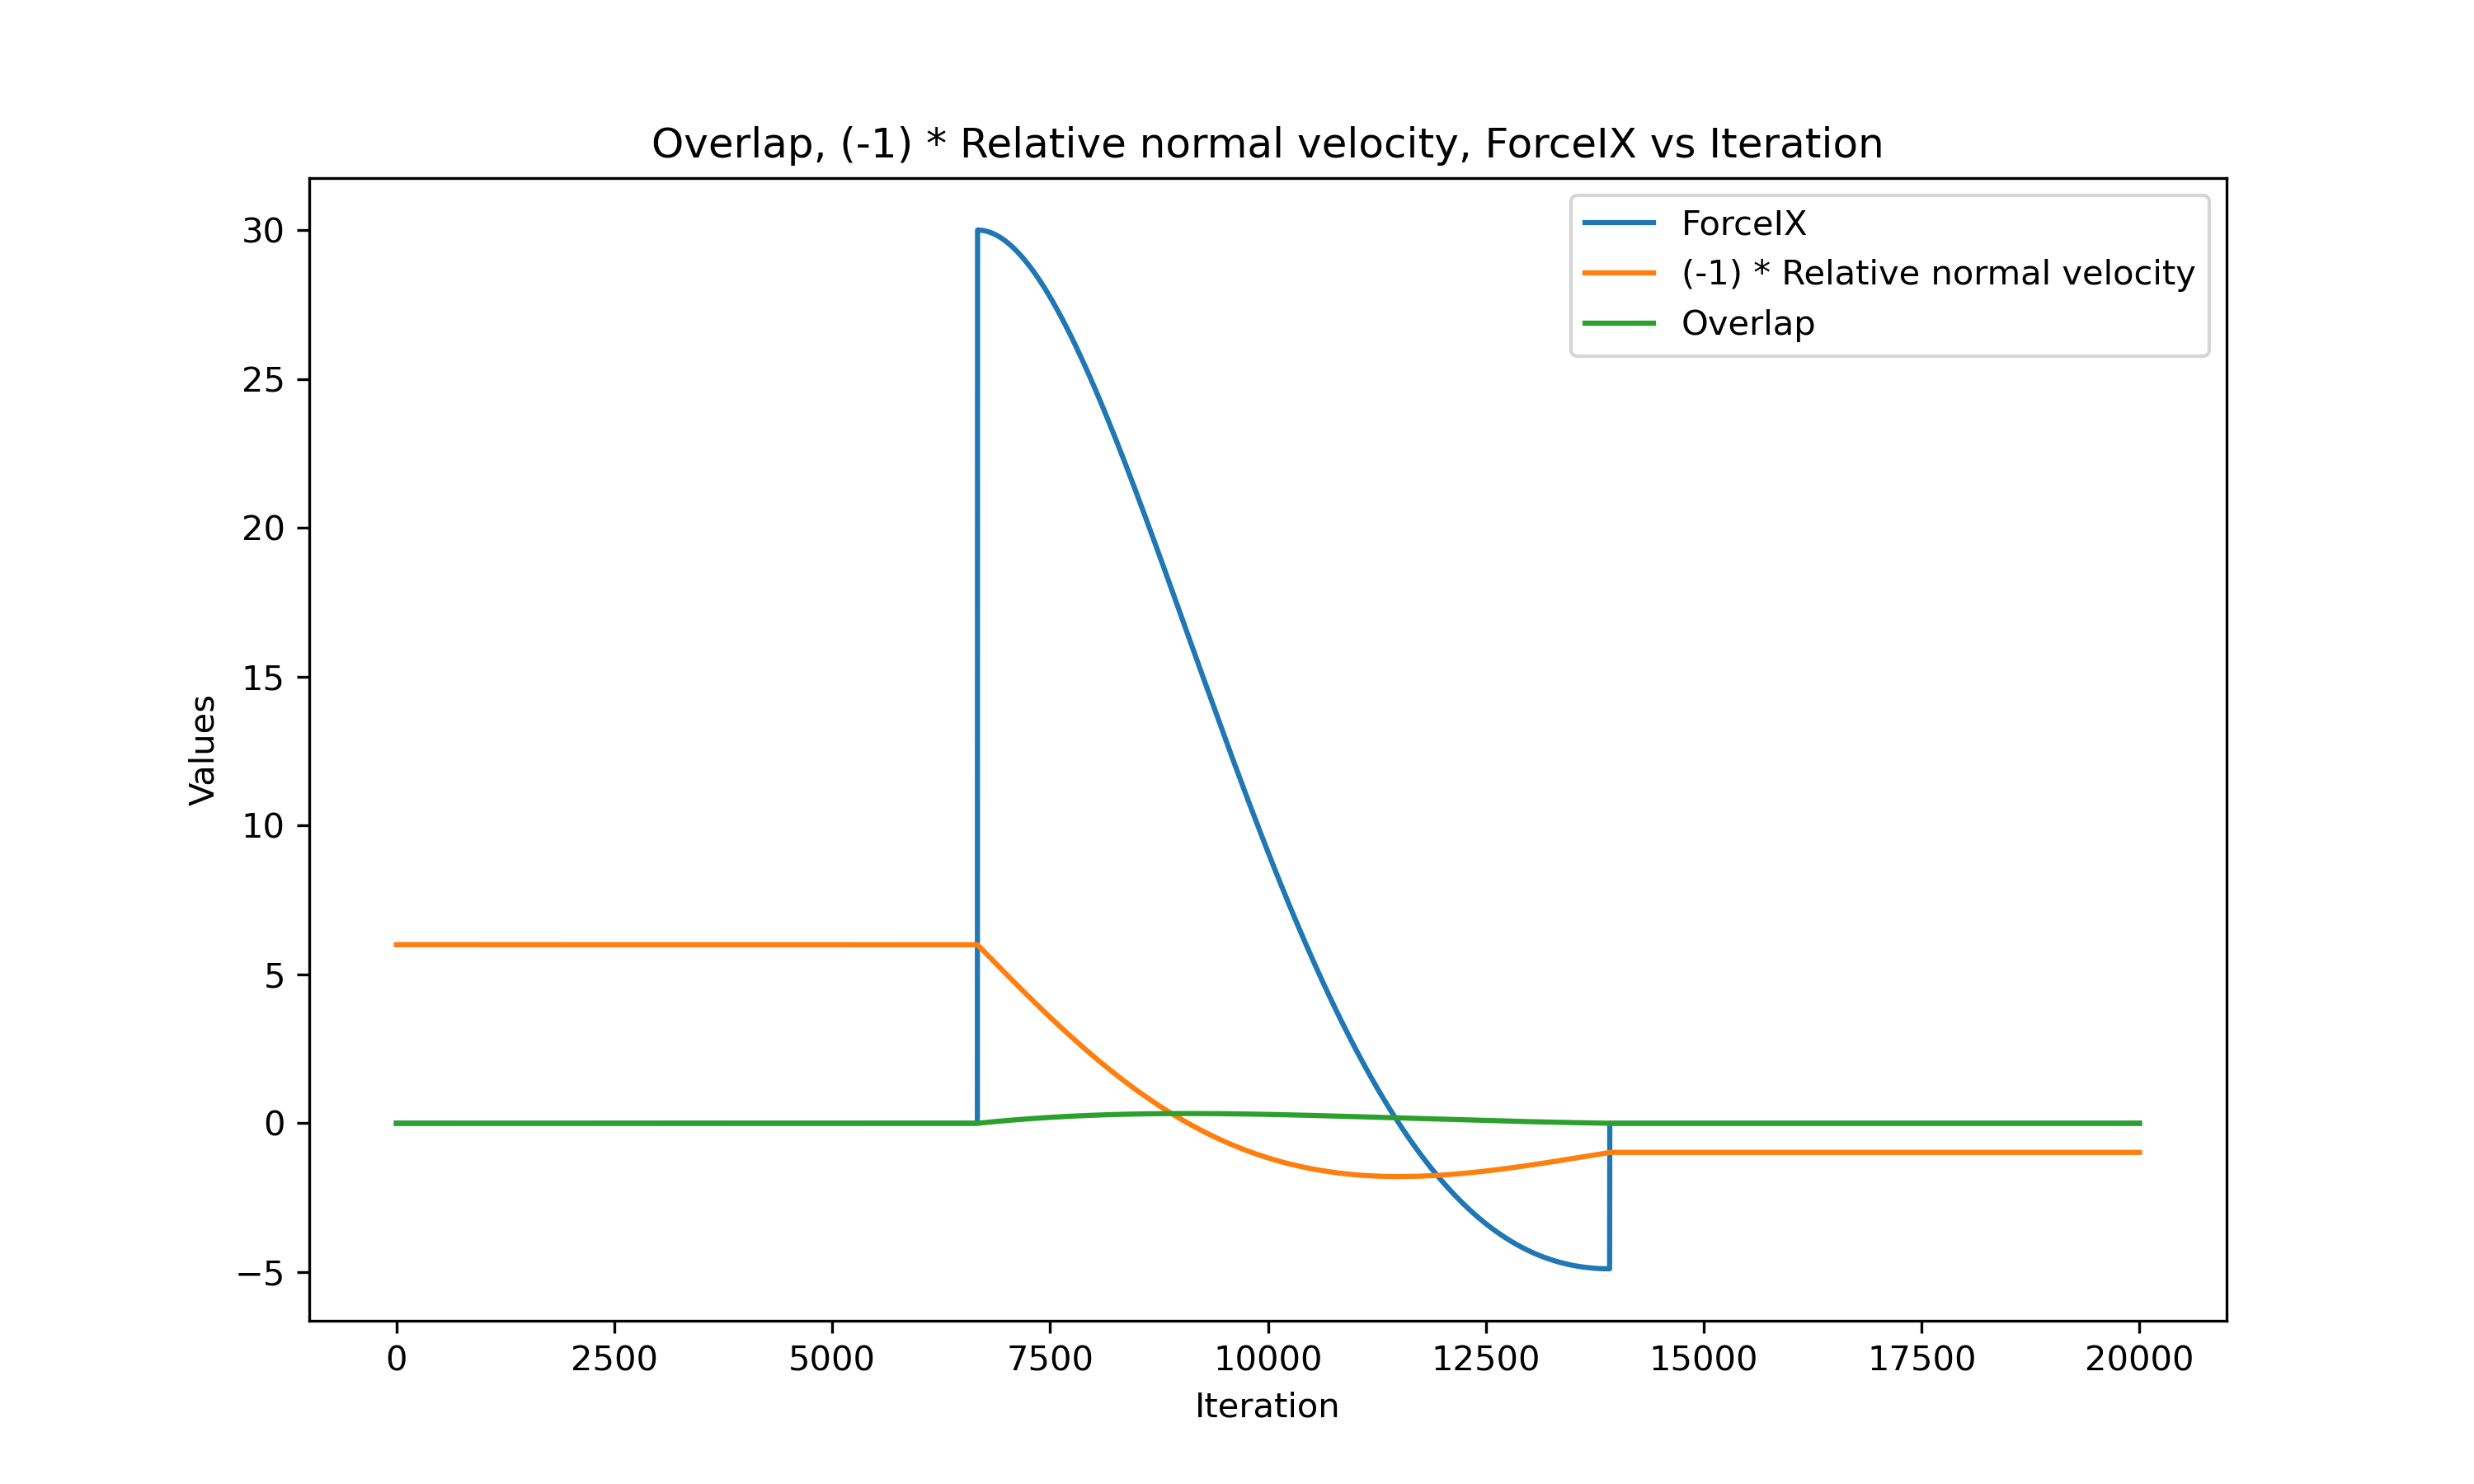
\includegraphics[width=0.65\textwidth]{figures/contactForceLaws/linearNormalContactModel/Overlap, Relative normal velocity vs Iteration simple_collision_two_particles_statistics_stiffness_50_viscosity_1e-2viscosity_5.png}
		\\ (b) $\gamma_n = 5$
	\end{center}
	
	% Shared caption
	\caption[Combined Caption]{Development of overlap ($\delta$), (-1) $\cdot$ relative normal velocity ($-v^n_{ji}$), force ($f^n_{ji}$) over time in scenario described in Figure~\ref{fig:combined_linear_normal_contact_model}.  Same parameter setting as in Figure~\ref{fig:Distance_Overlap_Force_plots}.}
	\label{fig:Relative_Normal_Velocity_plots}
\end{figure}


Figure~\ref{fig:combined_linear_normal_contact_model} and Figure~\ref{fig:Distance_Overlap_Force_plots} show a simple simulation to very the effect of the linear normal contact force.  Plot (a) and (b) of Figure~\ref{fig:Distance_Overlap_Force_plots} verify the repulsive effect of the force when the overlap is positive. As a consequence, the particles $i$ and $j$ move apart from each other in the normal direction, which can be observed in all cases with varying $\gamma_n$ .  
However, the variations in the normal viscosity coefficient $\gamma_n$ shows interesting effects. First, plot (b) suggests, cases with higher $\gamma_n$ experience lower maximum of overlap $\max(\delta)$, implying higher repulsion and deceleration. In the same context, in plot (a), cases with greater $\gamma_n$ show bigger differences between their velocities before ($v_{before}$) and after ($v_{after}$) the collision with decreasing ratio of $\frac{v_{after}}{v_{before}}$ for higher $\gamma_n$. Moreover, in plot (c), cases with high $\gamma_n \in$ \{0.5, 1, 5\} experience negative  / adhesive force at the end of their particle contacts (ca. Iteration $\in$ (12500, 13000) for $\gamma_n$ = 1). Similarly, cases with higher $\gamma_n$ show longer contact duration. This pulling force serves as a persuasive explanation for the higher deceleration effect for cases with higher $\gamma_n$.

These effects arise as the the dissipative force $f^n_{dissipative} = -\gamma_n \cdot v^n_{ji}$ becomes increasingly dominant due to higher $\gamma_n$, as Figure~\ref{fig:Relative_Normal_Velocity_plots} suggests. At the point of contact where $v_i$ changes its sign due to the repulsive normal force, the sign of relative velocity $v^n_{ij}$ changes too. As the term $-v^n_{ji}$ becomes negative, this can negatively affect the force and make it from repulsive to adhesive, if it is supported with high $\gamma_n$. Plus, great $f^n_{dissipative} = -\gamma_n \cdot v^n_{ji}$ also explains the abrupt increase of force $f^n_{ji}$ at the beginning of the contact of the particles.


These explanations of the observed phenomena are further supported by deriving the differential equation of the damped harmonic oscillator from Eqs.~\ref{equations_of_motion}, \ref{overlap_equation}, \ref{linear_normal_contact_model_equation1}, \ref{linear_normal_contact_model_equation2}, and \ref{linear_normal_contact_model_equation3}~\cite{Luding1998, Luding2008}:

\begin{align}
	\delta_{ji} &= (r_i + r_j) - \lVert \mathbf{x_i} - \mathbf{x_j} \rVert_2 \notag \\
	&= (r_i + r_j) - \frac{(\lVert \mathbf{x_i} - \mathbf{x_j} \rVert_2)^2}{\lVert \mathbf{x_i} - \mathbf{x_j} \rVert_2} \notag \\
	&= (r_i + r_j) - \frac{1}{\lVert \mathbf{x_i} - \mathbf{x_j} \rVert_2} 
	\cdot (\mathbf{x_i} - \mathbf{x_j}) \boldsymbol{\cdot} (\mathbf{x_i} - \mathbf{x_j}) \notag \\
	&= (r_i + r_j) - (\mathbf{x_i} - \mathbf{x_j}) \boldsymbol{\cdot} \mathbf{n_{ji}}.
	\label{overlap_reformulation}
\end{align}

Using Eq.~\ref{overlap_reformulation} to express \(f^n_{dissipative}\) gives:
\begin{align}
	f^n_{dissipative} &= -\gamma_n v^n_{ji} \notag \\
	&= -\gamma_n \cdot (\mathbf{v_i} - \mathbf{v_j}) \boldsymbol{\cdot} \mathbf{n_{ji}} \notag \\
	&= -\gamma_n \cdot \frac{\mathbf{x_i} - \mathbf{x_j}}{\lVert \mathbf{x_i} - \mathbf{x_j} \rVert_2} 
	\boldsymbol{\cdot} \frac{d}{dt}(\mathbf{x_i} - \mathbf{x_j}) \notag \\
	&= \gamma_n \cdot \left(-\frac{d}{dt} \lVert \mathbf{x_i} - \mathbf{x_j} \rVert_2\right) \notag \\
	&= \gamma_n \cdot \frac{d\delta_{ji}}{dt} \notag \\
	&= \gamma_n \cdot \dot{\delta}.
	\label{dissipative_force_reformulation}
\end{align}

Computing the second derivative of $\delta$ yields:
\begin{align}
	\ddot{\delta} &= -\frac{d}{dt}\big((\mathbf{v_i} - \mathbf{v_j}) \boldsymbol{\cdot} \mathbf{n_{ji}}\big) \notag \\
	&= -(\mathbf{\ddot{x}_i} - \mathbf{\ddot{x}_j}) \boldsymbol{\cdot} \mathbf{n_{ji}} \notag \\
	&= -\left(\frac{f^n_i}{m_i} - \frac{f^n_j}{m_j}\right), \quad \text{with} \quad 
	f^n_i = m_i \cdot (\mathbf{\ddot{x}_i} \boldsymbol{\cdot} \mathbf{n_{ji}}) \notag \\ 
	&= -\left(\frac{f^n_i}{m_i} + \frac{f^n_i}{m_j}\right), \quad \text{with} \quad 
	f^n_j = f^n_i \quad \text{(Newton's 3rd Law)} \notag \\
	&= -\frac{f^n_i}{m_{ij}}, \quad \text{with} \quad
	m_{ij} = \frac{m_i \cdot m_j}{(m_i + m_j)}.
	\label{second_derivative_of_overlap}
\end{align}

Inserting Eqs.~\ref{dissipative_force_reformulation} and \ref{linear_normal_contact_model_equation2} into \ref{second_derivative_of_overlap} results in:
\begin{align}
	\ddot{\delta} + \frac{f^n_i}{m_{ij}} &= \ddot{\delta} + \frac{f^n_{elastic} + f^n_{dissipative}}{m_{ij}} \notag \\
	&=  \ddot{\delta} + \frac{1}{m_{ij}} \cdot \left(k^n \cdot \delta + \gamma_n \cdot \dot{\delta}\right) \notag \\
	&= \ddot{\delta} + \frac{\gamma_n}{m_{ij}} \cdot \dot \delta + \frac{k^n}{m_{ij}} \cdot \delta \notag \\
	&= \ddot{\delta} + \frac{\gamma_n}{m_{ij}} \cdot \dot \delta + \frac{k^n}{m_{ij}} \cdot \delta \notag \\
	&= \ddot{\delta} + 2\eta\dot{\delta} + \omega_0^2\delta = 0, \quad \text{with} \quad \omega_0 = \sqrt{\frac{k^n}{m_{ij}}}, \quad \eta = \frac{\gamma_n}{2m_{ij}}.
\end{align}





\subsection{Long Range Normal Force Model}




\part{Implementation}

\part{Benchmarking}

\part{Fake Introduction and Background}
\chapter{Fake Introduction}
\label{sec:intro}       % labels can be put almost anywhere and can be referencef from anywhere.
Write some useful intro. Here are tips along the way:

\section{Tips}
\subsection{How to Describe}
% optional: set the spacing between columns
\setlength{\columnsep}{30 pt}
When listing several points you have three basic options:
\begin{multicols}{3}
    \begin{itemize}
        \item itemize
        \item enumerate
        \item description
    \end{itemize}

    \vfill\null
    \columnbreak

    \begin{enumerate}
        \item itemize
        \item enumerate
        \item description
    \end{enumerate}

    \vfill\null
    \columnbreak

    \begin{description}
        \item[itemize] short, unordered
        \item[enumerate] short ordered
        \item[description] listing of descriptions. Also nice for longer ones.
    \end{description}

\end{multicols}


\subsection{How to Quote}

\begin{quote}
    "This is a quote!"
\end{quote}

\begin{itemize}
    \item Citations to a source can be made like this \verb|\cite{gratl17task}| =~\cite{gratl17task}
    \subitem Always join text and the citation with a non-breaking space: \verb|text~\cite{foo}|.
    \item Referencing Sections, Figures, Tables, Formulas: \verb|\autoref{sec:intro}| = \autoref{sec:intro}.
    \item Footnotes for url or further notes: \verb|\footnote{\url{https://www.top500.org}}| = \footnote{\url{https://www.top500.org}}
\end{itemize}

\subsection{How to Math}

Use the align environment for equations especially if you want to align them somehow.

\begin{align}
1 + 1 &\ne 3\\
\left(\dfrac{10}{1}\right) - 9 &= 1
\end{align}

% if you need a pagebreak because figure placement is broken:
\clearpage

\section{Environments}

\subsection{How to Figure}

Anything can also be put in multiple columns.

\begin{multicols}{2} % defines an environment with two columns
    \begin{figure}[H] % [H] for HERE
        \centering
        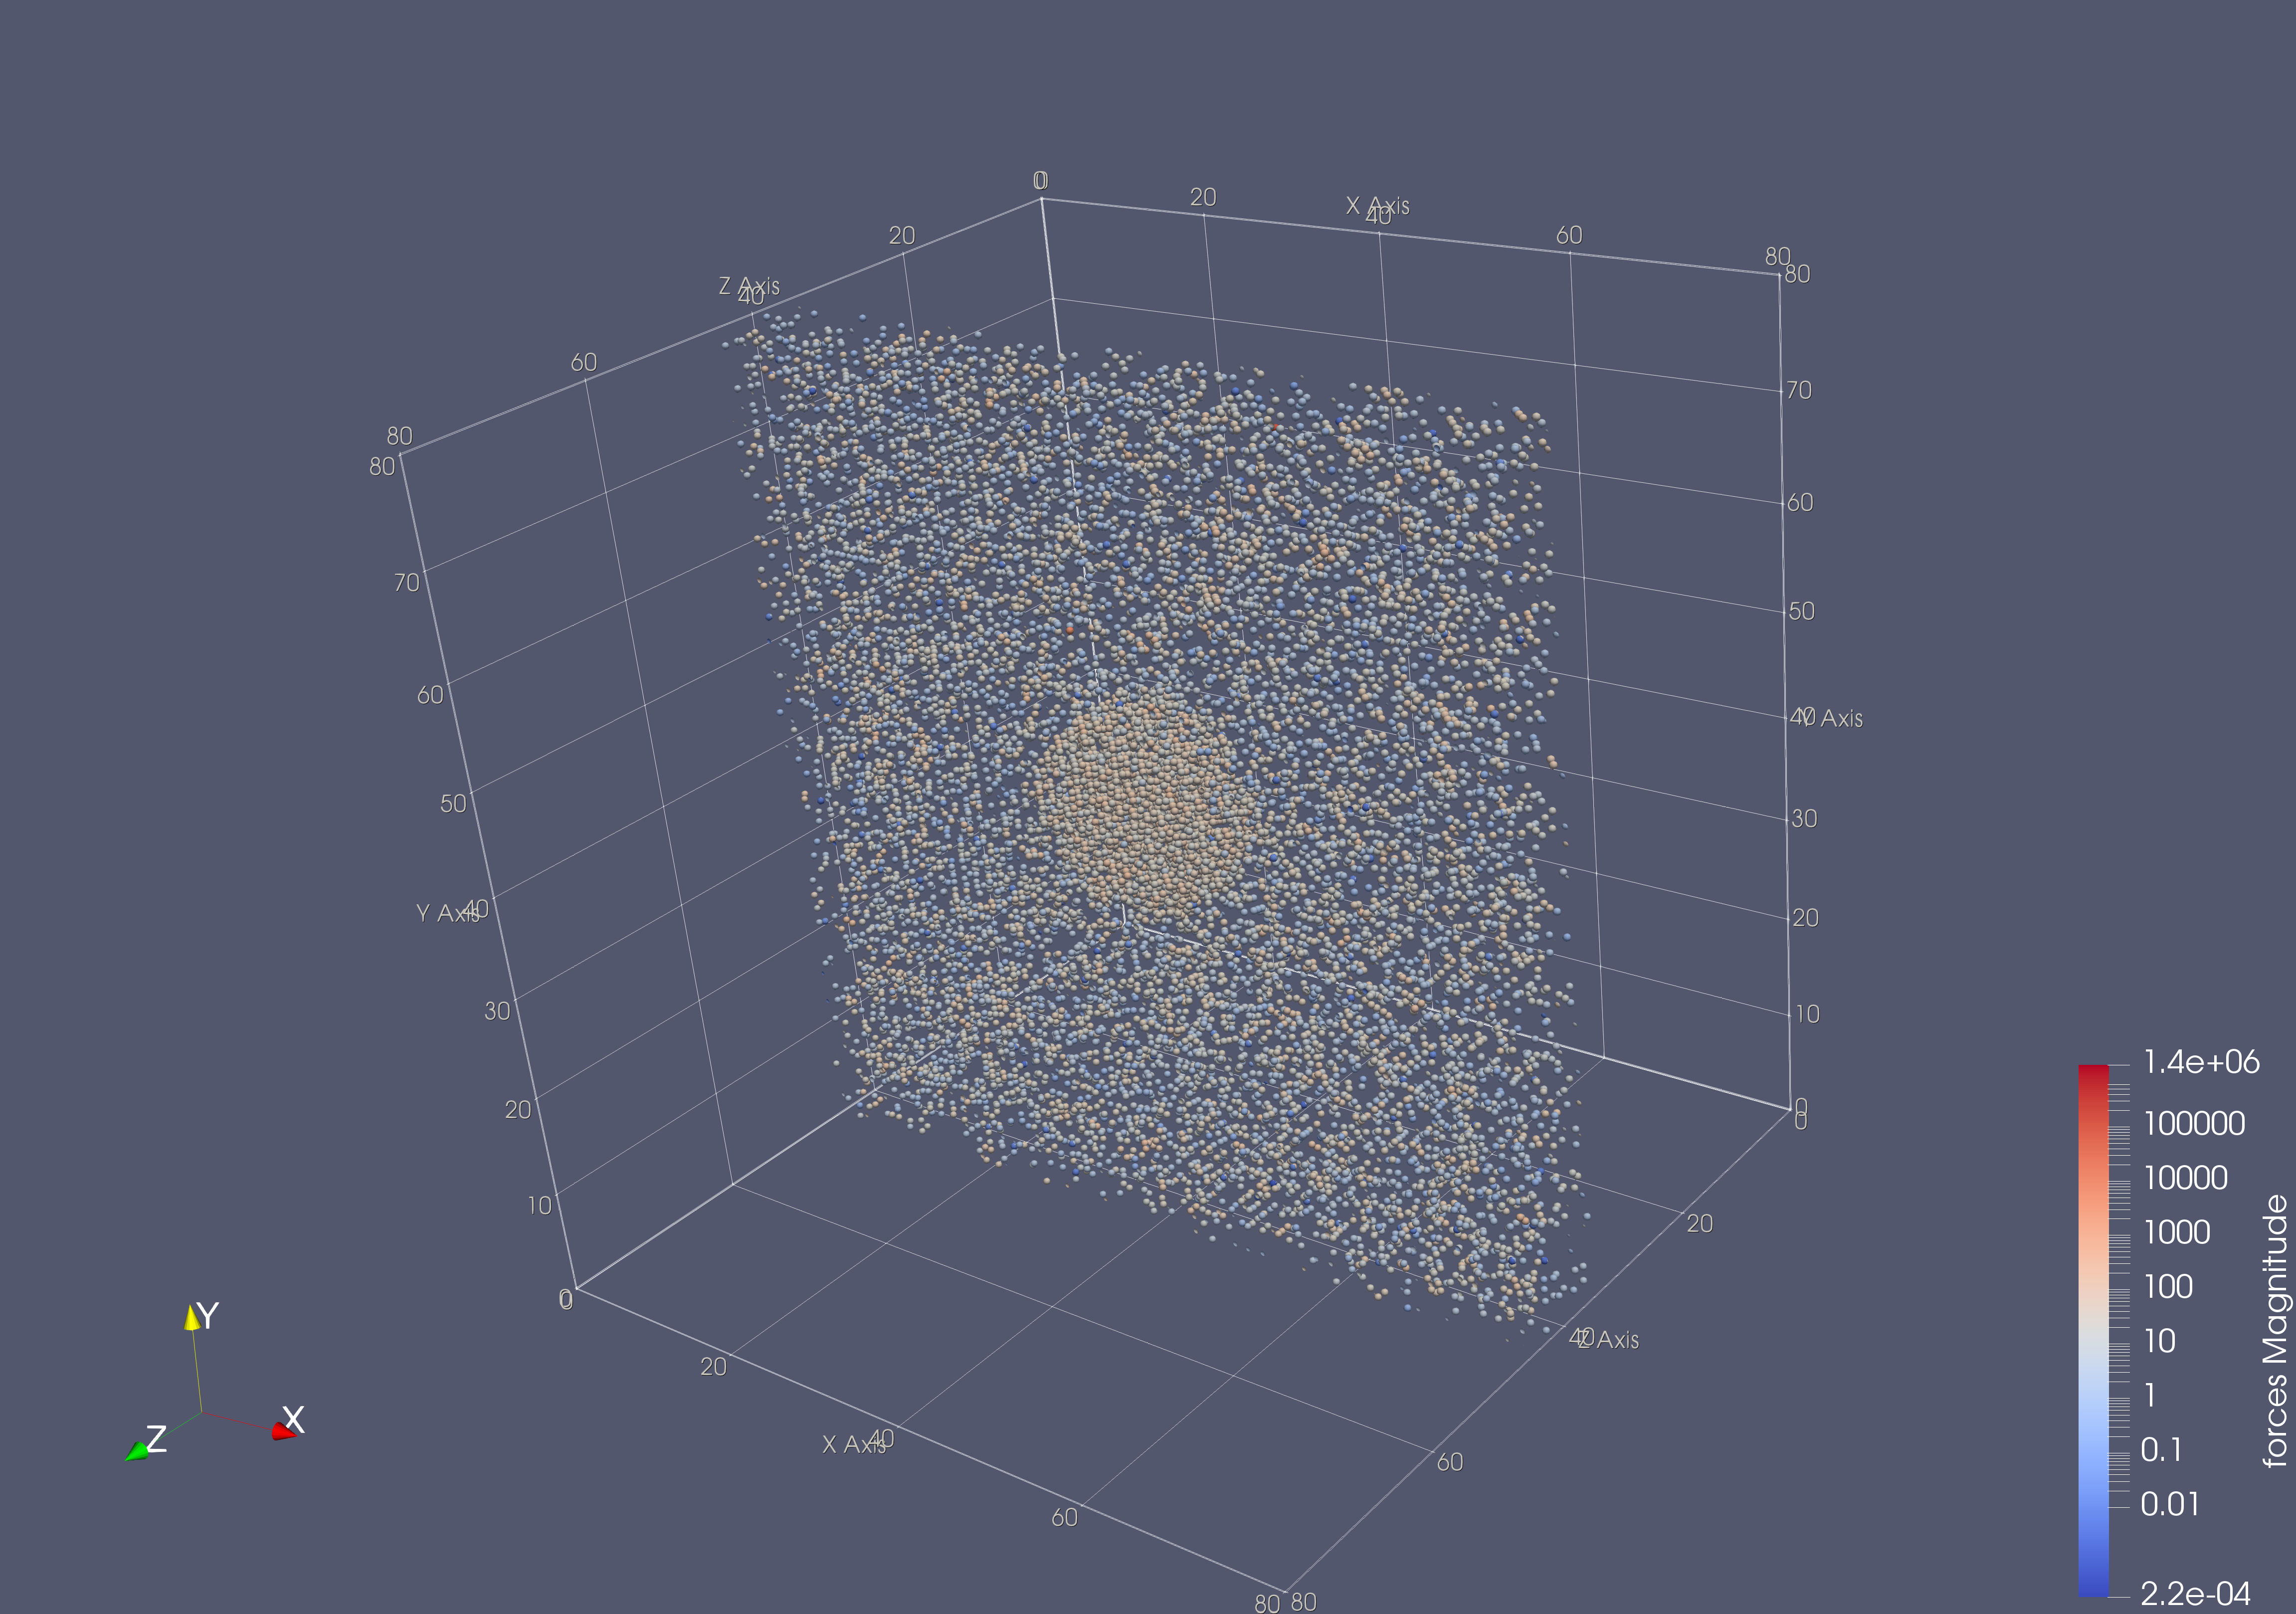
\includegraphics[width=.9\columnwidth]{figures/scenario_clip_rot.png}
        \caption[Example Figure]{Some Caption. Always also include a source if it wasn't created by you!\\
            \tiny{Source: \cite{gratl17task}}}
        \label{fig:exampleLabel1} % labels always have to be placed after the caption
    \end{figure}

    \columnbreak    % start next column

    \begin{figure}[H]
        \centering
        \begin{tikzpicture}
            \node[anchor=south west,inner sep=0] (image) at (0,0) {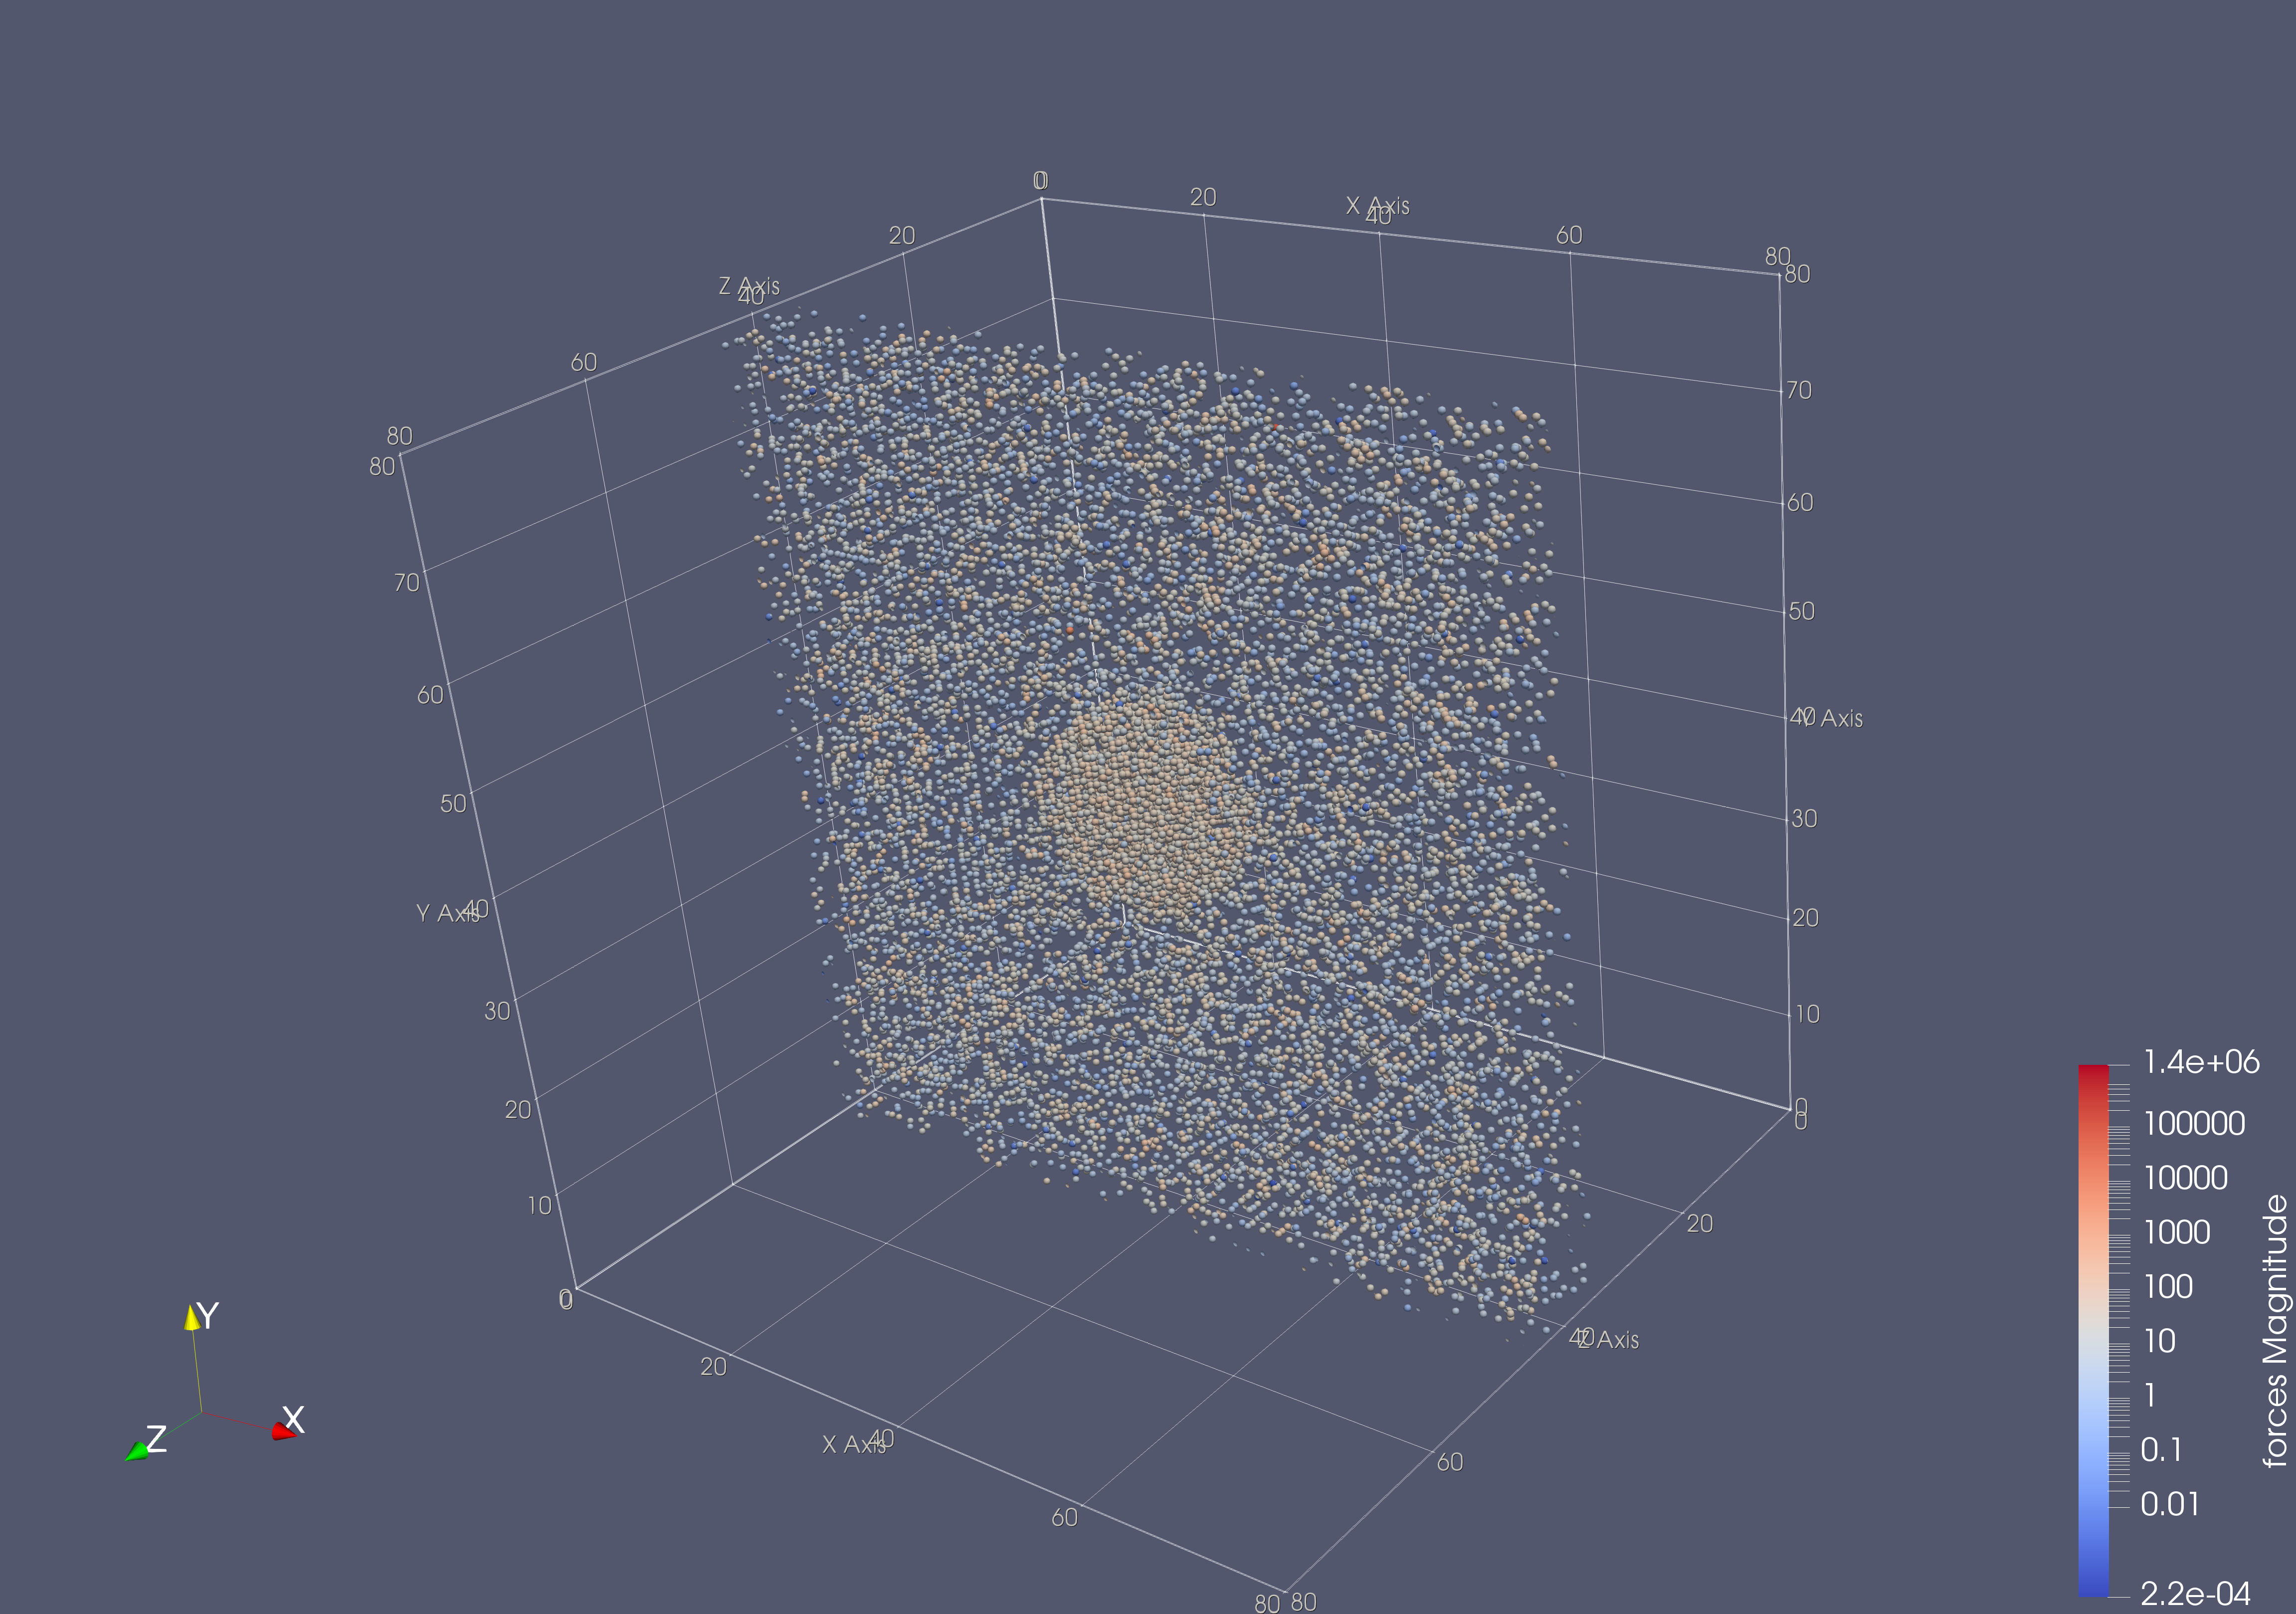
\includegraphics[width=.9\columnwidth]{figures/scenario_clip_rot.png}};
            \begin{scope}[x={(image.south east)},y={(image.north west)}]
            \draw[red, thin,rounded corners] (.42,.42) rectangle (.58,.6);
            \end{scope}
        \end{tikzpicture}
        \caption[Figure with tikz]{Figures can be drawn on or completely generated with tikz.}
        \label{fig:exampleLabel2}
    \end{figure}
\end{multicols}

\paragraph{Subfigures}
If grouping of several pictures seems reasonable, think about using subfigures. This often comes in handy with plots.

\begin{figure}[H]
    \centering
    \begin{subfigure}[b]{0.33\textwidth}
        \includegraphics[width=\textwidth]{example-image-a}
        \caption{example-image-a}
        \label{fig:example-image-a}
    \end{subfigure}
    \begin{subfigure}[b]{0.33\textwidth}
        \includegraphics[width=\textwidth]{example-image-b}
        \caption{example-image-b}
        \label{fig:example-image-b}
    \end{subfigure}
    \begin{subfigure}[b]{0.33\textwidth}
        \includegraphics[width=\textwidth]{example-image-c}
        \caption{example-image-c}
        \label{fig:example-image-c}
    \end{subfigure}
    \caption{One caption to describe them all.}
\end{figure}

\subsection{How to Algorithm}

\begin{figure}
\begin{algorithm}[H]

% Define custom keywords
\SetKwFunction{KwNot}{not}
% Define custom Functions
\SetKwFunction{Fissorted}{is\_sorted}
\SetKwFunction{Fbogosort}{bogosort}
\SetKwFunction{Fshuffle}{shuffle}
\SetKwProg{Fn}{Function}{:}{}
\KwIn{\tabto{2cm}data array}
\KwOut{\tabto{2cm} data sorted}
\BlankLine

\tcp{Checks if array is sorted}
\Fn{\Fissorted{data}}{
    \For{i $\leftarrow$ 0 \KwTo data.size() - 1}{
    \label{algo:for}            % labels can also be put in the algorithm
        \If{data[i] $>$ data[i+1]}{
            \Return false
        }
    }
    \Return true
}

\tcp{actual algorithm}
\Fn{\Fbogosort{data}}{
    \While{\KwNot \Fissorted{data}}{
        random.\Fshuffle{data}
    }
}

\caption[Bogosort]{Bogosort}
\label{algo:example}
\end{algorithm}
\caption{some description what is happening}
\end{figure}

\clearpage

\subsection{How to Code}
\begin{lstlisting}[style=eclipse-cpp, caption=General form of a typical runner() function., label=code:runner]
void runner(int type, void *data){
    switch(type)
        case taskType1:
            // do stuff using data
        case taskType2:
            // do other stuff using data
}
\end{lstlisting}

\subsection{How to Table}
\begin{table}[H]
    \begin{tabularx}{\columnwidth}{L | C | R}
        \hline
        \hline
        bla left & bla centered\newline over two lines &  bla right\\
        \hline
        bla left & bla centered & \multirow[c]{2}{\hsize}{cell spanning two rows} \\
        \cline{1-2}
        \multicolumn{2}{c|}{cell spanning two columns} & \\
    \end{tabularx}
    \caption[Some Table]{Fancy table that can contain line breaks and extended cells.}
    \label{tab:example}
\end{table}

\appendix
\part{Appendix}
\chapter{Some more stuff}

For everything that does not really belong in the thesis but is good to mention.

\listoffigures

\listoftables

\bibliographystyle{alpha}
\bibliography{literature}

\end{document}
